
\subsection{Numerical solution}

In this section we present the numerical solution of problem \eqref{eq:diagonal_case_cauchy_problem} for several Péclet numbers. The width and height of the domain are $L = 1 \ \meter$ and the velocity of the flow is $u = 1 \ \meter / \second$. The density is kept constant at $\rho = 1000 \ \kilo\gram / \meter^3$, therefore Péclet's number is varied by chaging the diffusion coefficient $\Gamma$. The boundary conditions are $\phi_\text{low} = 0$ and $\phi_\text{high} = 1$. A uniform mesh of $N = 200$ nodes has been used to discretize the domain, with a tolerance of $10^{-12}$ as a stop criterion for the Gauss--Seidel algorithm. The Upwind--Difference Scheme (UDS) has been chosen to compute the convective properties.

Figure \ref{fig:diagonal_N200_Pe1.0e+00} shows the solution to the diagonal case problem for $\peclet = 1$. Transport and diffusion have a similar strength as can be seen in the central zone of the domain $\Omega$. There is clearly a transport phenomena carrying the fluid from the lower left corner to the upper right corner of $\Omega$, but there is also mixing due to the diffusion process. Note that the solution is not continuous at the lower left and upper right corners because of the sudden jump from $\phi_\text{low}$ to $\phi_\text{high}$. The zone around the upper left corner does not seem affected by the diffusion process as it is far from the boundary where $\phi = \phi_\text{low}$. The same applies to the zone close to the lower right corner.

\begin{figure}[h]
	\centering
	\vspace{-0.75cm}
%	\fbox{% GNUPLOT: LaTeX picture with Postscript
\documentclass{minimal}
% Set font size
\makeatletter
\def\@ptsize{1}
\InputIfFileExists{size11.clo}{}{%
   \GenericError{(gnuplot) \space\space\space\@spaces}{%
      Gnuplot Error: File `size11.clo' not found! Could not set font size%
   }{See the gnuplot documentation for explanation.%
   }{For using a font size a file `size<fontsize>.clo' has to exist.
        Falling back ^^Jto default fontsize 10pt.}%
  \def\@ptsize{0}
  \input{size10.clo}%
}%
\makeatother
% Load packages
\usepackage{calc}
\usepackage{graphicx}
\usepackage{color}
\usepackage[cp1252]{inputenc}
\makeatletter
% Select an appropriate default driver (from TeXLive graphics.cfg)
\begingroup
  \chardef\x=0 %
  % check pdfTeX
  \@ifundefined{pdfoutput}{}{%
    \ifcase\pdfoutput
    \else
      \chardef\x=1 %
    \fi
  }%
  % check VTeX
  \@ifundefined{OpMode}{}{%
    \chardef\x=2 %
  }%
\expandafter\endgroup
\ifcase\x
  % default case
  \PassOptionsToPackage{dvips}{geometry}
\or
  % pdfTeX is running in pdf mode
  \PassOptionsToPackage{pdftex}{geometry}
\else
  % VTeX is running
  \PassOptionsToPackage{vtex}{geometry}
\fi
\makeatother
% Set papersize
\usepackage[papersize={340.10bp,340.10bp},text={340.10bp,340.10bp}]{geometry}
% No page numbers and no paragraph indentation
\pagestyle{empty}
\setlength{\parindent}{0bp}%
% Load configuration file
\InputIfFileExists{gnuplot.cfg}{%
  \typeout{Using configuration file gnuplot.cfg}%
}{%
 \typeout{No configuration file gnuplot.cfg found.}%
}%
%
\begin{document}
\begingroup
  % Encoding inside the plot.  In the header of your document, this encoding
  % should to defined, e.g., by using
  % \usepackage[cp1252,<other encodings>]{inputenc}
  \inputencoding{cp1252}%
  \makeatletter
  \providecommand\color[2][]{%
    \GenericError{(gnuplot) \space\space\space\@spaces}{%
      Package color not loaded in conjunction with
      terminal option `colourtext'%
    }{See the gnuplot documentation for explanation.%
    }{Either use 'blacktext' in gnuplot or load the package
      color.sty in LaTeX.}%
    \renewcommand\color[2][]{}%
  }%
  \providecommand\includegraphics[2][]{%
    \GenericError{(gnuplot) \space\space\space\@spaces}{%
      Package graphicx or graphics not loaded%
    }{See the gnuplot documentation for explanation.%
    }{The gnuplot epslatex terminal needs graphicx.sty or graphics.sty.}%
    \renewcommand\includegraphics[2][]{}%
  }%
  \providecommand\rotatebox[2]{#2}%
  \@ifundefined{ifGPcolor}{%
    \newif\ifGPcolor
    \GPcolortrue
  }{}%
  \@ifundefined{ifGPblacktext}{%
    \newif\ifGPblacktext
    \GPblacktextfalse
  }{}%
  % define a \g@addto@macro without @ in the name:
  \let\gplgaddtomacro\g@addto@macro
  % define empty templates for all commands taking text:
  \gdef\gplbacktext{}%
  \gdef\gplfronttext{}%
  \makeatother
  \ifGPblacktext
    % no textcolor at all
    \def\colorrgb#1{}%
    \def\colorgray#1{}%
  \else
    % gray or color?
    \ifGPcolor
      \def\colorrgb#1{\color[rgb]{#1}}%
      \def\colorgray#1{\color[gray]{#1}}%
      \expandafter\def\csname LTw\endcsname{\color{white}}%
      \expandafter\def\csname LTb\endcsname{\color{black}}%
      \expandafter\def\csname LTa\endcsname{\color{black}}%
      \expandafter\def\csname LT0\endcsname{\color[rgb]{1,0,0}}%
      \expandafter\def\csname LT1\endcsname{\color[rgb]{0,1,0}}%
      \expandafter\def\csname LT2\endcsname{\color[rgb]{0,0,1}}%
      \expandafter\def\csname LT3\endcsname{\color[rgb]{1,0,1}}%
      \expandafter\def\csname LT4\endcsname{\color[rgb]{0,1,1}}%
      \expandafter\def\csname LT5\endcsname{\color[rgb]{1,1,0}}%
      \expandafter\def\csname LT6\endcsname{\color[rgb]{0,0,0}}%
      \expandafter\def\csname LT7\endcsname{\color[rgb]{1,0.3,0}}%
      \expandafter\def\csname LT8\endcsname{\color[rgb]{0.5,0.5,0.5}}%
    \else
      % gray
      \def\colorrgb#1{\color{black}}%
      \def\colorgray#1{\color[gray]{#1}}%
      \expandafter\def\csname LTw\endcsname{\color{white}}%
      \expandafter\def\csname LTb\endcsname{\color{black}}%
      \expandafter\def\csname LTa\endcsname{\color{black}}%
      \expandafter\def\csname LT0\endcsname{\color{black}}%
      \expandafter\def\csname LT1\endcsname{\color{black}}%
      \expandafter\def\csname LT2\endcsname{\color{black}}%
      \expandafter\def\csname LT3\endcsname{\color{black}}%
      \expandafter\def\csname LT4\endcsname{\color{black}}%
      \expandafter\def\csname LT5\endcsname{\color{black}}%
      \expandafter\def\csname LT6\endcsname{\color{black}}%
      \expandafter\def\csname LT7\endcsname{\color{black}}%
      \expandafter\def\csname LT8\endcsname{\color{black}}%
    \fi
  \fi
    \setlength{\unitlength}{0.0500bp}%
    \ifx\gptboxheight\undefined%
      \newlength{\gptboxheight}%
      \newlength{\gptboxwidth}%
      \newsavebox{\gptboxtext}%
    \fi%
    \setlength{\fboxrule}{0.5pt}%
    \setlength{\fboxsep}{1pt}%
    \definecolor{tbcol}{rgb}{1,1,1}%
\begin{picture}(6802.00,6802.00)%
    \gplgaddtomacro\gplbacktext{%
      \csname LTb\endcsname%%
      \put(814,1105){\makebox(0,0)[r]{\strut{}0.0}}%
      \put(814,2032){\makebox(0,0)[r]{\strut{}0.2}}%
      \put(814,2959){\makebox(0,0)[r]{\strut{}0.4}}%
      \put(814,3886){\makebox(0,0)[r]{\strut{}0.6}}%
      \put(814,4813){\makebox(0,0)[r]{\strut{}0.8}}%
      \put(814,5740){\makebox(0,0)[r]{\strut{}1.0}}%
      \put(946,885){\makebox(0,0){\strut{}0.0}}%
      \put(1873,885){\makebox(0,0){\strut{}0.2}}%
      \put(2800,885){\makebox(0,0){\strut{}0.4}}%
      \put(3727,885){\makebox(0,0){\strut{}0.6}}%
      \put(4654,885){\makebox(0,0){\strut{}0.8}}%
      \put(5581,885){\makebox(0,0){\strut{}1.0}}%
    }%
    \gplgaddtomacro\gplfronttext{%
      \csname LTb\endcsname%%
      \put(209,3422){\rotatebox{-270}{\makebox(0,0){\strut{}$y \ (\mathrm{m})$}}}%
      \put(3263,555){\makebox(0,0){\strut{}$x \ (\mathrm{m})$}}%
      \csname LTb\endcsname%%
      \put(6060,1105){\makebox(0,0)[l]{\strut{}0.0}}%
      \put(6060,2032){\makebox(0,0)[l]{\strut{}0.2}}%
      \put(6060,2959){\makebox(0,0)[l]{\strut{}0.4}}%
      \put(6060,3886){\makebox(0,0)[l]{\strut{}0.6}}%
      \put(6060,4813){\makebox(0,0)[l]{\strut{}0.8}}%
      \put(6060,5740){\makebox(0,0)[l]{\strut{}1.0}}%
      \put(6522,3422){\rotatebox{-270}{\makebox(0,0){\strut{}$\phi$}}}%
      \put(3263,6070){\makebox(0,0){\strut{}\textbf{Diagonal case} $(\mathrm{Pe} = 1)$}}%
    }%
    \gplbacktext
    \put(0,0){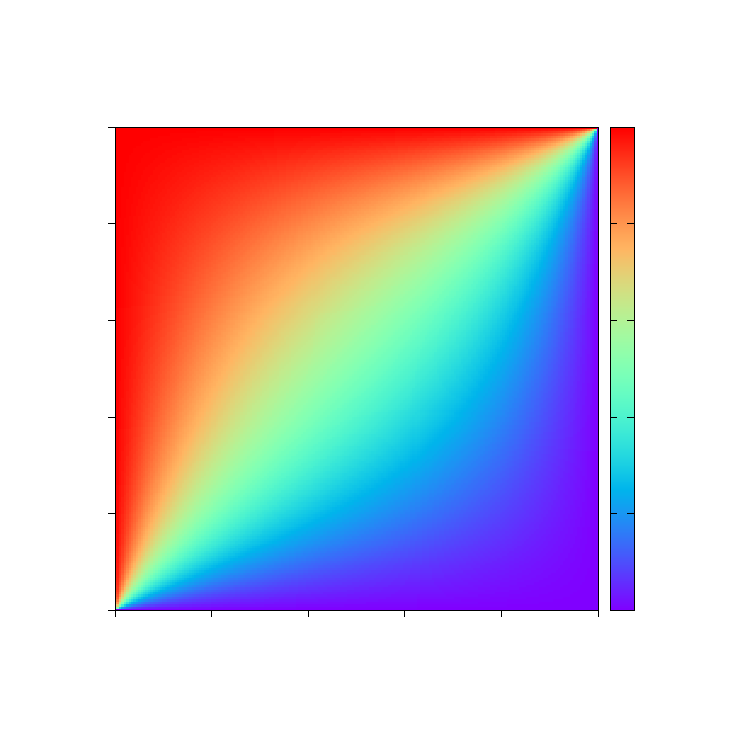
\includegraphics[width={340.10bp},height={340.10bp}]{diagonal_N200_Pe1.0e+00-inc}}%
    \gplfronttext
  \end{picture}%
\endgroup
\end{document}
}
	% GNUPLOT: LaTeX picture with Postscript
\documentclass{minimal}
% Set font size
\makeatletter
\def\@ptsize{1}
\InputIfFileExists{size11.clo}{}{%
   \GenericError{(gnuplot) \space\space\space\@spaces}{%
      Gnuplot Error: File `size11.clo' not found! Could not set font size%
   }{See the gnuplot documentation for explanation.%
   }{For using a font size a file `size<fontsize>.clo' has to exist.
        Falling back ^^Jto default fontsize 10pt.}%
  \def\@ptsize{0}
  \input{size10.clo}%
}%
\makeatother
% Load packages
\usepackage{calc}
\usepackage{graphicx}
\usepackage{color}
\usepackage[cp1252]{inputenc}
\makeatletter
% Select an appropriate default driver (from TeXLive graphics.cfg)
\begingroup
  \chardef\x=0 %
  % check pdfTeX
  \@ifundefined{pdfoutput}{}{%
    \ifcase\pdfoutput
    \else
      \chardef\x=1 %
    \fi
  }%
  % check VTeX
  \@ifundefined{OpMode}{}{%
    \chardef\x=2 %
  }%
\expandafter\endgroup
\ifcase\x
  % default case
  \PassOptionsToPackage{dvips}{geometry}
\or
  % pdfTeX is running in pdf mode
  \PassOptionsToPackage{pdftex}{geometry}
\else
  % VTeX is running
  \PassOptionsToPackage{vtex}{geometry}
\fi
\makeatother
% Set papersize
\usepackage[papersize={340.10bp,340.10bp},text={340.10bp,340.10bp}]{geometry}
% No page numbers and no paragraph indentation
\pagestyle{empty}
\setlength{\parindent}{0bp}%
% Load configuration file
\InputIfFileExists{gnuplot.cfg}{%
  \typeout{Using configuration file gnuplot.cfg}%
}{%
 \typeout{No configuration file gnuplot.cfg found.}%
}%
%
\begin{document}
\begingroup
  % Encoding inside the plot.  In the header of your document, this encoding
  % should to defined, e.g., by using
  % \usepackage[cp1252,<other encodings>]{inputenc}
  \inputencoding{cp1252}%
  \makeatletter
  \providecommand\color[2][]{%
    \GenericError{(gnuplot) \space\space\space\@spaces}{%
      Package color not loaded in conjunction with
      terminal option `colourtext'%
    }{See the gnuplot documentation for explanation.%
    }{Either use 'blacktext' in gnuplot or load the package
      color.sty in LaTeX.}%
    \renewcommand\color[2][]{}%
  }%
  \providecommand\includegraphics[2][]{%
    \GenericError{(gnuplot) \space\space\space\@spaces}{%
      Package graphicx or graphics not loaded%
    }{See the gnuplot documentation for explanation.%
    }{The gnuplot epslatex terminal needs graphicx.sty or graphics.sty.}%
    \renewcommand\includegraphics[2][]{}%
  }%
  \providecommand\rotatebox[2]{#2}%
  \@ifundefined{ifGPcolor}{%
    \newif\ifGPcolor
    \GPcolortrue
  }{}%
  \@ifundefined{ifGPblacktext}{%
    \newif\ifGPblacktext
    \GPblacktextfalse
  }{}%
  % define a \g@addto@macro without @ in the name:
  \let\gplgaddtomacro\g@addto@macro
  % define empty templates for all commands taking text:
  \gdef\gplbacktext{}%
  \gdef\gplfronttext{}%
  \makeatother
  \ifGPblacktext
    % no textcolor at all
    \def\colorrgb#1{}%
    \def\colorgray#1{}%
  \else
    % gray or color?
    \ifGPcolor
      \def\colorrgb#1{\color[rgb]{#1}}%
      \def\colorgray#1{\color[gray]{#1}}%
      \expandafter\def\csname LTw\endcsname{\color{white}}%
      \expandafter\def\csname LTb\endcsname{\color{black}}%
      \expandafter\def\csname LTa\endcsname{\color{black}}%
      \expandafter\def\csname LT0\endcsname{\color[rgb]{1,0,0}}%
      \expandafter\def\csname LT1\endcsname{\color[rgb]{0,1,0}}%
      \expandafter\def\csname LT2\endcsname{\color[rgb]{0,0,1}}%
      \expandafter\def\csname LT3\endcsname{\color[rgb]{1,0,1}}%
      \expandafter\def\csname LT4\endcsname{\color[rgb]{0,1,1}}%
      \expandafter\def\csname LT5\endcsname{\color[rgb]{1,1,0}}%
      \expandafter\def\csname LT6\endcsname{\color[rgb]{0,0,0}}%
      \expandafter\def\csname LT7\endcsname{\color[rgb]{1,0.3,0}}%
      \expandafter\def\csname LT8\endcsname{\color[rgb]{0.5,0.5,0.5}}%
    \else
      % gray
      \def\colorrgb#1{\color{black}}%
      \def\colorgray#1{\color[gray]{#1}}%
      \expandafter\def\csname LTw\endcsname{\color{white}}%
      \expandafter\def\csname LTb\endcsname{\color{black}}%
      \expandafter\def\csname LTa\endcsname{\color{black}}%
      \expandafter\def\csname LT0\endcsname{\color{black}}%
      \expandafter\def\csname LT1\endcsname{\color{black}}%
      \expandafter\def\csname LT2\endcsname{\color{black}}%
      \expandafter\def\csname LT3\endcsname{\color{black}}%
      \expandafter\def\csname LT4\endcsname{\color{black}}%
      \expandafter\def\csname LT5\endcsname{\color{black}}%
      \expandafter\def\csname LT6\endcsname{\color{black}}%
      \expandafter\def\csname LT7\endcsname{\color{black}}%
      \expandafter\def\csname LT8\endcsname{\color{black}}%
    \fi
  \fi
    \setlength{\unitlength}{0.0500bp}%
    \ifx\gptboxheight\undefined%
      \newlength{\gptboxheight}%
      \newlength{\gptboxwidth}%
      \newsavebox{\gptboxtext}%
    \fi%
    \setlength{\fboxrule}{0.5pt}%
    \setlength{\fboxsep}{1pt}%
    \definecolor{tbcol}{rgb}{1,1,1}%
\begin{picture}(6802.00,6802.00)%
    \gplgaddtomacro\gplbacktext{%
      \csname LTb\endcsname%%
      \put(814,1105){\makebox(0,0)[r]{\strut{}0.0}}%
      \put(814,2032){\makebox(0,0)[r]{\strut{}0.2}}%
      \put(814,2959){\makebox(0,0)[r]{\strut{}0.4}}%
      \put(814,3886){\makebox(0,0)[r]{\strut{}0.6}}%
      \put(814,4813){\makebox(0,0)[r]{\strut{}0.8}}%
      \put(814,5740){\makebox(0,0)[r]{\strut{}1.0}}%
      \put(946,885){\makebox(0,0){\strut{}0.0}}%
      \put(1873,885){\makebox(0,0){\strut{}0.2}}%
      \put(2800,885){\makebox(0,0){\strut{}0.4}}%
      \put(3727,885){\makebox(0,0){\strut{}0.6}}%
      \put(4654,885){\makebox(0,0){\strut{}0.8}}%
      \put(5581,885){\makebox(0,0){\strut{}1.0}}%
    }%
    \gplgaddtomacro\gplfronttext{%
      \csname LTb\endcsname%%
      \put(209,3422){\rotatebox{-270}{\makebox(0,0){\strut{}$y \ (\mathrm{m})$}}}%
      \put(3263,555){\makebox(0,0){\strut{}$x \ (\mathrm{m})$}}%
      \csname LTb\endcsname%%
      \put(6060,1105){\makebox(0,0)[l]{\strut{}0.0}}%
      \put(6060,2032){\makebox(0,0)[l]{\strut{}0.2}}%
      \put(6060,2959){\makebox(0,0)[l]{\strut{}0.4}}%
      \put(6060,3886){\makebox(0,0)[l]{\strut{}0.6}}%
      \put(6060,4813){\makebox(0,0)[l]{\strut{}0.8}}%
      \put(6060,5740){\makebox(0,0)[l]{\strut{}1.0}}%
      \put(6522,3422){\rotatebox{-270}{\makebox(0,0){\strut{}$\phi$}}}%
      \put(3263,6070){\makebox(0,0){\strut{}\textbf{Diagonal case} $(\mathrm{Pe} = 1)$}}%
    }%
    \gplbacktext
    \put(0,0){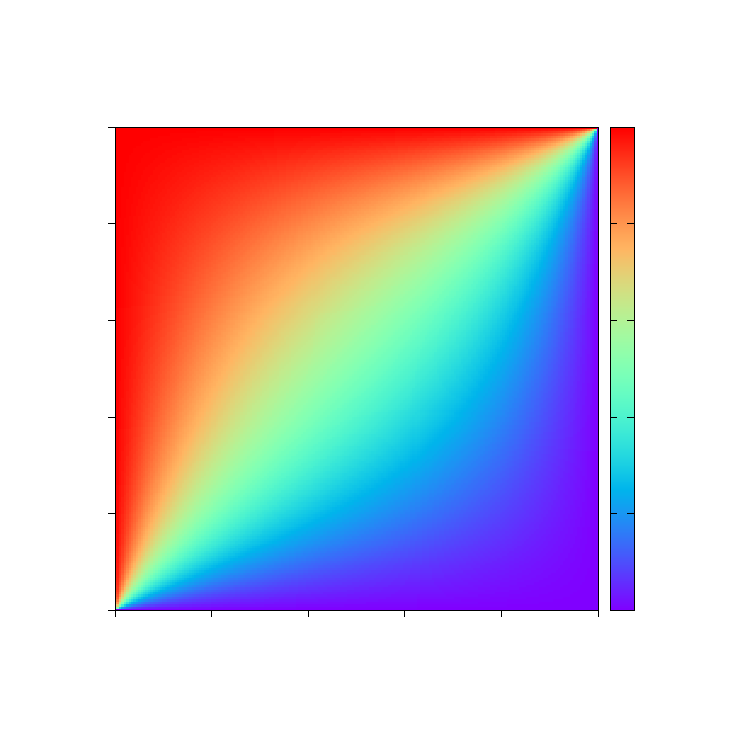
\includegraphics[width={340.10bp},height={340.10bp}]{diagonal_N200_Pe1.0e+00-inc}}%
    \gplfronttext
  \end{picture}%
\endgroup
\end{document}

	\vspace{-0.50cm}
	\caption{Numerical solution to the diagonal case for $\peclet = 1$.}
	\label{fig:diagonal_N200_Pe1.0e+00}
\end{figure}

\clearpage
Figures \eqref{fig:diagonal_N200_Pe1.0e+01} to \eqref{fig:diagonal_N200_Pe1.0e+04} show the diagonal case solution for $\peclet = 10, \ 10^2, \ 10^4$ and $10^9$. The solution for $\peclet = 10$ (figure \ref{fig:diagonal_N200_Pe1.0e+01}) has a similar appearance to the solution for $\peclet = 1$ (figure \ref{fig:diagonal_N200_Pe1.0e+00}). As Péclet's number grows, the transport process takes over the diffusion process. Therefore the diffusion zone, which is centered in the diagonal along the fluid flow, tends to shrink. This change in the behaviour of the solution can be observed by comparing the cases for $\peclet = 10$ (figure \ref{fig:diagonal_N200_Pe1.0e+01}) and $\peclet = 10^2$ (figure \ref{fig:diagonal_N200_Pe1.0e+02}). For $\peclet = 10^4$ the diffusion zone becomes even narrower. Beyond $\peclet = 10^4$ there are no obvious changes in the solution, as can be checked by looking at the case for $\peclet = 10^9$ (figure \ref{fig:diagonal_N200_Pe1.0e+09}).

\begin{figure}[h]
	\centering
	\begin{subfigure}{.5\textwidth}
		\centering
		\vspace{-0.75cm}
%		\fbox{% GNUPLOT: LaTeX picture with Postscript
\begingroup
  % Encoding inside the plot.  In the header of your document, this encoding
  % should to defined, e.g., by using
  % \usepackage[cp1252,<other encodings>]{inputenc}
  \inputencoding{cp1252}%
  \makeatletter
  \providecommand\color[2][]{%
    \GenericError{(gnuplot) \space\space\space\@spaces}{%
      Package color not loaded in conjunction with
      terminal option `colourtext'%
    }{See the gnuplot documentation for explanation.%
    }{Either use 'blacktext' in gnuplot or load the package
      color.sty in LaTeX.}%
    \renewcommand\color[2][]{}%
  }%
  \providecommand\includegraphics[2][]{%
    \GenericError{(gnuplot) \space\space\space\@spaces}{%
      Package graphicx or graphics not loaded%
    }{See the gnuplot documentation for explanation.%
    }{The gnuplot epslatex terminal needs graphicx.sty or graphics.sty.}%
    \renewcommand\includegraphics[2][]{}%
  }%
  \providecommand\rotatebox[2]{#2}%
  \@ifundefined{ifGPcolor}{%
    \newif\ifGPcolor
    \GPcolortrue
  }{}%
  \@ifundefined{ifGPblacktext}{%
    \newif\ifGPblacktext
    \GPblacktextfalse
  }{}%
  % define a \g@addto@macro without @ in the name:
  \let\gplgaddtomacro\g@addto@macro
  % define empty templates for all commands taking text:
  \gdef\gplbacktext{}%
  \gdef\gplfronttext{}%
  \makeatother
  \ifGPblacktext
    % no textcolor at all
    \def\colorrgb#1{}%
    \def\colorgray#1{}%
  \else
    % gray or color?
    \ifGPcolor
      \def\colorrgb#1{\color[rgb]{#1}}%
      \def\colorgray#1{\color[gray]{#1}}%
      \expandafter\def\csname LTw\endcsname{\color{white}}%
      \expandafter\def\csname LTb\endcsname{\color{black}}%
      \expandafter\def\csname LTa\endcsname{\color{black}}%
      \expandafter\def\csname LT0\endcsname{\color[rgb]{1,0,0}}%
      \expandafter\def\csname LT1\endcsname{\color[rgb]{0,1,0}}%
      \expandafter\def\csname LT2\endcsname{\color[rgb]{0,0,1}}%
      \expandafter\def\csname LT3\endcsname{\color[rgb]{1,0,1}}%
      \expandafter\def\csname LT4\endcsname{\color[rgb]{0,1,1}}%
      \expandafter\def\csname LT5\endcsname{\color[rgb]{1,1,0}}%
      \expandafter\def\csname LT6\endcsname{\color[rgb]{0,0,0}}%
      \expandafter\def\csname LT7\endcsname{\color[rgb]{1,0.3,0}}%
      \expandafter\def\csname LT8\endcsname{\color[rgb]{0.5,0.5,0.5}}%
    \else
      % gray
      \def\colorrgb#1{\color{black}}%
      \def\colorgray#1{\color[gray]{#1}}%
      \expandafter\def\csname LTw\endcsname{\color{white}}%
      \expandafter\def\csname LTb\endcsname{\color{black}}%
      \expandafter\def\csname LTa\endcsname{\color{black}}%
      \expandafter\def\csname LT0\endcsname{\color{black}}%
      \expandafter\def\csname LT1\endcsname{\color{black}}%
      \expandafter\def\csname LT2\endcsname{\color{black}}%
      \expandafter\def\csname LT3\endcsname{\color{black}}%
      \expandafter\def\csname LT4\endcsname{\color{black}}%
      \expandafter\def\csname LT5\endcsname{\color{black}}%
      \expandafter\def\csname LT6\endcsname{\color{black}}%
      \expandafter\def\csname LT7\endcsname{\color{black}}%
      \expandafter\def\csname LT8\endcsname{\color{black}}%
    \fi
  \fi
    \setlength{\unitlength}{0.0500bp}%
    \ifx\gptboxheight\undefined%
      \newlength{\gptboxheight}%
      \newlength{\gptboxwidth}%
      \newsavebox{\gptboxtext}%
    \fi%
    \setlength{\fboxrule}{0.5pt}%
    \setlength{\fboxsep}{1pt}%
    \definecolor{tbcol}{rgb}{1,1,1}%
\begin{picture}(4534.00,4534.00)%
    \gplgaddtomacro\gplbacktext{%
      \csname LTb\endcsname%%
      \put(814,991){\makebox(0,0)[r]{\strut{}0.0}}%
      \put(814,1510){\makebox(0,0)[r]{\strut{}0.2}}%
      \put(814,2029){\makebox(0,0)[r]{\strut{}0.4}}%
      \put(814,2548){\makebox(0,0)[r]{\strut{}0.6}}%
      \put(814,3067){\makebox(0,0)[r]{\strut{}0.8}}%
      \put(814,3586){\makebox(0,0)[r]{\strut{}1.0}}%
      \put(946,771){\makebox(0,0){\strut{}0.0}}%
      \put(1465,771){\makebox(0,0){\strut{}0.2}}%
      \put(1984,771){\makebox(0,0){\strut{}0.4}}%
      \put(2502,771){\makebox(0,0){\strut{}0.6}}%
      \put(3021,771){\makebox(0,0){\strut{}0.8}}%
      \put(3540,771){\makebox(0,0){\strut{}1.0}}%
    }%
    \gplgaddtomacro\gplfronttext{%
      \csname LTb\endcsname%%
      \put(209,2288){\rotatebox{-270}{\makebox(0,0){\strut{}$y \ (\mathrm{m})$}}}%
      \put(2243,441){\makebox(0,0){\strut{}$x \ (\mathrm{m})$}}%
      \csname LTb\endcsname%%
      \put(3866,991){\makebox(0,0)[l]{\strut{}0.0}}%
      \put(3866,1510){\makebox(0,0)[l]{\strut{}0.2}}%
      \put(3866,2029){\makebox(0,0)[l]{\strut{}0.4}}%
      \put(3866,2548){\makebox(0,0)[l]{\strut{}0.6}}%
      \put(3866,3067){\makebox(0,0)[l]{\strut{}0.8}}%
      \put(3866,3586){\makebox(0,0)[l]{\strut{}1.0}}%
      \put(4328,2288){\rotatebox{-270}{\makebox(0,0){\strut{}$\phi$}}}%
      \put(2243,3916){\makebox(0,0){\strut{}\textbf{Diagonal case} $(\peclet = 10)$}}%
    }%
    \gplbacktext
    \put(0,0){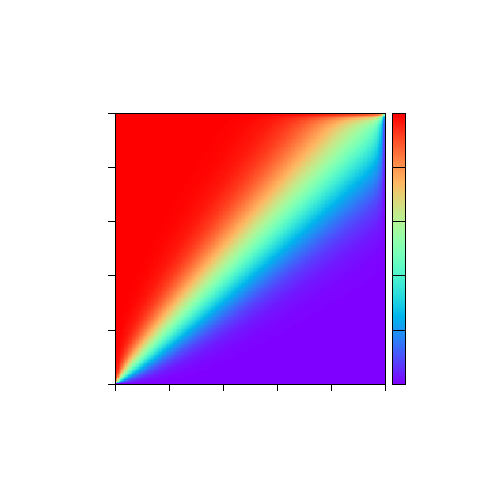
\includegraphics[width={226.70bp},height={226.70bp}]{figures/case_diagonal_flow/diagonal_N200_Pe1.0e+01}}%
    \gplfronttext
  \end{picture}%
\endgroup
}
		% GNUPLOT: LaTeX picture with Postscript
\begingroup
  % Encoding inside the plot.  In the header of your document, this encoding
  % should to defined, e.g., by using
  % \usepackage[cp1252,<other encodings>]{inputenc}
  \inputencoding{cp1252}%
  \makeatletter
  \providecommand\color[2][]{%
    \GenericError{(gnuplot) \space\space\space\@spaces}{%
      Package color not loaded in conjunction with
      terminal option `colourtext'%
    }{See the gnuplot documentation for explanation.%
    }{Either use 'blacktext' in gnuplot or load the package
      color.sty in LaTeX.}%
    \renewcommand\color[2][]{}%
  }%
  \providecommand\includegraphics[2][]{%
    \GenericError{(gnuplot) \space\space\space\@spaces}{%
      Package graphicx or graphics not loaded%
    }{See the gnuplot documentation for explanation.%
    }{The gnuplot epslatex terminal needs graphicx.sty or graphics.sty.}%
    \renewcommand\includegraphics[2][]{}%
  }%
  \providecommand\rotatebox[2]{#2}%
  \@ifundefined{ifGPcolor}{%
    \newif\ifGPcolor
    \GPcolortrue
  }{}%
  \@ifundefined{ifGPblacktext}{%
    \newif\ifGPblacktext
    \GPblacktextfalse
  }{}%
  % define a \g@addto@macro without @ in the name:
  \let\gplgaddtomacro\g@addto@macro
  % define empty templates for all commands taking text:
  \gdef\gplbacktext{}%
  \gdef\gplfronttext{}%
  \makeatother
  \ifGPblacktext
    % no textcolor at all
    \def\colorrgb#1{}%
    \def\colorgray#1{}%
  \else
    % gray or color?
    \ifGPcolor
      \def\colorrgb#1{\color[rgb]{#1}}%
      \def\colorgray#1{\color[gray]{#1}}%
      \expandafter\def\csname LTw\endcsname{\color{white}}%
      \expandafter\def\csname LTb\endcsname{\color{black}}%
      \expandafter\def\csname LTa\endcsname{\color{black}}%
      \expandafter\def\csname LT0\endcsname{\color[rgb]{1,0,0}}%
      \expandafter\def\csname LT1\endcsname{\color[rgb]{0,1,0}}%
      \expandafter\def\csname LT2\endcsname{\color[rgb]{0,0,1}}%
      \expandafter\def\csname LT3\endcsname{\color[rgb]{1,0,1}}%
      \expandafter\def\csname LT4\endcsname{\color[rgb]{0,1,1}}%
      \expandafter\def\csname LT5\endcsname{\color[rgb]{1,1,0}}%
      \expandafter\def\csname LT6\endcsname{\color[rgb]{0,0,0}}%
      \expandafter\def\csname LT7\endcsname{\color[rgb]{1,0.3,0}}%
      \expandafter\def\csname LT8\endcsname{\color[rgb]{0.5,0.5,0.5}}%
    \else
      % gray
      \def\colorrgb#1{\color{black}}%
      \def\colorgray#1{\color[gray]{#1}}%
      \expandafter\def\csname LTw\endcsname{\color{white}}%
      \expandafter\def\csname LTb\endcsname{\color{black}}%
      \expandafter\def\csname LTa\endcsname{\color{black}}%
      \expandafter\def\csname LT0\endcsname{\color{black}}%
      \expandafter\def\csname LT1\endcsname{\color{black}}%
      \expandafter\def\csname LT2\endcsname{\color{black}}%
      \expandafter\def\csname LT3\endcsname{\color{black}}%
      \expandafter\def\csname LT4\endcsname{\color{black}}%
      \expandafter\def\csname LT5\endcsname{\color{black}}%
      \expandafter\def\csname LT6\endcsname{\color{black}}%
      \expandafter\def\csname LT7\endcsname{\color{black}}%
      \expandafter\def\csname LT8\endcsname{\color{black}}%
    \fi
  \fi
    \setlength{\unitlength}{0.0500bp}%
    \ifx\gptboxheight\undefined%
      \newlength{\gptboxheight}%
      \newlength{\gptboxwidth}%
      \newsavebox{\gptboxtext}%
    \fi%
    \setlength{\fboxrule}{0.5pt}%
    \setlength{\fboxsep}{1pt}%
    \definecolor{tbcol}{rgb}{1,1,1}%
\begin{picture}(4534.00,4534.00)%
    \gplgaddtomacro\gplbacktext{%
      \csname LTb\endcsname%%
      \put(814,991){\makebox(0,0)[r]{\strut{}0.0}}%
      \put(814,1510){\makebox(0,0)[r]{\strut{}0.2}}%
      \put(814,2029){\makebox(0,0)[r]{\strut{}0.4}}%
      \put(814,2548){\makebox(0,0)[r]{\strut{}0.6}}%
      \put(814,3067){\makebox(0,0)[r]{\strut{}0.8}}%
      \put(814,3586){\makebox(0,0)[r]{\strut{}1.0}}%
      \put(946,771){\makebox(0,0){\strut{}0.0}}%
      \put(1465,771){\makebox(0,0){\strut{}0.2}}%
      \put(1984,771){\makebox(0,0){\strut{}0.4}}%
      \put(2502,771){\makebox(0,0){\strut{}0.6}}%
      \put(3021,771){\makebox(0,0){\strut{}0.8}}%
      \put(3540,771){\makebox(0,0){\strut{}1.0}}%
    }%
    \gplgaddtomacro\gplfronttext{%
      \csname LTb\endcsname%%
      \put(209,2288){\rotatebox{-270}{\makebox(0,0){\strut{}$y \ (\mathrm{m})$}}}%
      \put(2243,441){\makebox(0,0){\strut{}$x \ (\mathrm{m})$}}%
      \csname LTb\endcsname%%
      \put(3866,991){\makebox(0,0)[l]{\strut{}0.0}}%
      \put(3866,1510){\makebox(0,0)[l]{\strut{}0.2}}%
      \put(3866,2029){\makebox(0,0)[l]{\strut{}0.4}}%
      \put(3866,2548){\makebox(0,0)[l]{\strut{}0.6}}%
      \put(3866,3067){\makebox(0,0)[l]{\strut{}0.8}}%
      \put(3866,3586){\makebox(0,0)[l]{\strut{}1.0}}%
      \put(4328,2288){\rotatebox{-270}{\makebox(0,0){\strut{}$\phi$}}}%
      \put(2243,3916){\makebox(0,0){\strut{}\textbf{Diagonal case} $(\peclet = 10)$}}%
    }%
    \gplbacktext
    \put(0,0){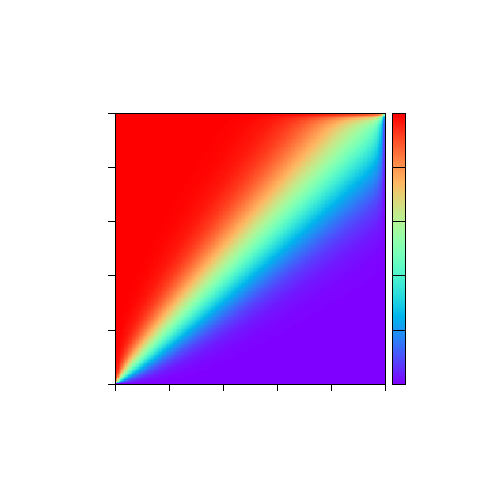
\includegraphics[width={226.70bp},height={226.70bp}]{figures/case_diagonal_flow/diagonal_N200_Pe1.0e+01}}%
    \gplfronttext
  \end{picture}%
\endgroup

		\vspace{-0.50cm}
		\captionsetup{width=0.8\textwidth}
		\caption{Numerical solution to the diagonal case for $\peclet = 10$.}
		\label{fig:diagonal_N200_Pe1.0e+01}
	\end{subfigure}%
	\begin{subfigure}{.5\textwidth}
		\centering
		\vspace{-0.75cm}
%		\fbox{% GNUPLOT: LaTeX picture with Postscript
\begingroup
  % Encoding inside the plot.  In the header of your document, this encoding
  % should to defined, e.g., by using
  % \usepackage[cp1252,<other encodings>]{inputenc}
  \inputencoding{cp1252}%
  \makeatletter
  \providecommand\color[2][]{%
    \GenericError{(gnuplot) \space\space\space\@spaces}{%
      Package color not loaded in conjunction with
      terminal option `colourtext'%
    }{See the gnuplot documentation for explanation.%
    }{Either use 'blacktext' in gnuplot or load the package
      color.sty in LaTeX.}%
    \renewcommand\color[2][]{}%
  }%
  \providecommand\includegraphics[2][]{%
    \GenericError{(gnuplot) \space\space\space\@spaces}{%
      Package graphicx or graphics not loaded%
    }{See the gnuplot documentation for explanation.%
    }{The gnuplot epslatex terminal needs graphicx.sty or graphics.sty.}%
    \renewcommand\includegraphics[2][]{}%
  }%
  \providecommand\rotatebox[2]{#2}%
  \@ifundefined{ifGPcolor}{%
    \newif\ifGPcolor
    \GPcolortrue
  }{}%
  \@ifundefined{ifGPblacktext}{%
    \newif\ifGPblacktext
    \GPblacktextfalse
  }{}%
  % define a \g@addto@macro without @ in the name:
  \let\gplgaddtomacro\g@addto@macro
  % define empty templates for all commands taking text:
  \gdef\gplbacktext{}%
  \gdef\gplfronttext{}%
  \makeatother
  \ifGPblacktext
    % no textcolor at all
    \def\colorrgb#1{}%
    \def\colorgray#1{}%
  \else
    % gray or color?
    \ifGPcolor
      \def\colorrgb#1{\color[rgb]{#1}}%
      \def\colorgray#1{\color[gray]{#1}}%
      \expandafter\def\csname LTw\endcsname{\color{white}}%
      \expandafter\def\csname LTb\endcsname{\color{black}}%
      \expandafter\def\csname LTa\endcsname{\color{black}}%
      \expandafter\def\csname LT0\endcsname{\color[rgb]{1,0,0}}%
      \expandafter\def\csname LT1\endcsname{\color[rgb]{0,1,0}}%
      \expandafter\def\csname LT2\endcsname{\color[rgb]{0,0,1}}%
      \expandafter\def\csname LT3\endcsname{\color[rgb]{1,0,1}}%
      \expandafter\def\csname LT4\endcsname{\color[rgb]{0,1,1}}%
      \expandafter\def\csname LT5\endcsname{\color[rgb]{1,1,0}}%
      \expandafter\def\csname LT6\endcsname{\color[rgb]{0,0,0}}%
      \expandafter\def\csname LT7\endcsname{\color[rgb]{1,0.3,0}}%
      \expandafter\def\csname LT8\endcsname{\color[rgb]{0.5,0.5,0.5}}%
    \else
      % gray
      \def\colorrgb#1{\color{black}}%
      \def\colorgray#1{\color[gray]{#1}}%
      \expandafter\def\csname LTw\endcsname{\color{white}}%
      \expandafter\def\csname LTb\endcsname{\color{black}}%
      \expandafter\def\csname LTa\endcsname{\color{black}}%
      \expandafter\def\csname LT0\endcsname{\color{black}}%
      \expandafter\def\csname LT1\endcsname{\color{black}}%
      \expandafter\def\csname LT2\endcsname{\color{black}}%
      \expandafter\def\csname LT3\endcsname{\color{black}}%
      \expandafter\def\csname LT4\endcsname{\color{black}}%
      \expandafter\def\csname LT5\endcsname{\color{black}}%
      \expandafter\def\csname LT6\endcsname{\color{black}}%
      \expandafter\def\csname LT7\endcsname{\color{black}}%
      \expandafter\def\csname LT8\endcsname{\color{black}}%
    \fi
  \fi
    \setlength{\unitlength}{0.0500bp}%
    \ifx\gptboxheight\undefined%
      \newlength{\gptboxheight}%
      \newlength{\gptboxwidth}%
      \newsavebox{\gptboxtext}%
    \fi%
    \setlength{\fboxrule}{0.5pt}%
    \setlength{\fboxsep}{1pt}%
    \definecolor{tbcol}{rgb}{1,1,1}%
\begin{picture}(4534.00,4534.00)%
    \gplgaddtomacro\gplbacktext{%
      \csname LTb\endcsname%%
      \put(814,991){\makebox(0,0)[r]{\strut{}0.0}}%
      \put(814,1510){\makebox(0,0)[r]{\strut{}0.2}}%
      \put(814,2029){\makebox(0,0)[r]{\strut{}0.4}}%
      \put(814,2548){\makebox(0,0)[r]{\strut{}0.6}}%
      \put(814,3067){\makebox(0,0)[r]{\strut{}0.8}}%
      \put(814,3586){\makebox(0,0)[r]{\strut{}1.0}}%
      \put(946,771){\makebox(0,0){\strut{}0.0}}%
      \put(1465,771){\makebox(0,0){\strut{}0.2}}%
      \put(1984,771){\makebox(0,0){\strut{}0.4}}%
      \put(2502,771){\makebox(0,0){\strut{}0.6}}%
      \put(3021,771){\makebox(0,0){\strut{}0.8}}%
      \put(3540,771){\makebox(0,0){\strut{}1.0}}%
    }%
    \gplgaddtomacro\gplfronttext{%
      \csname LTb\endcsname%%
      \put(209,2288){\rotatebox{-270}{\makebox(0,0){\strut{}$y \ (\mathrm{m})$}}}%
      \put(2243,441){\makebox(0,0){\strut{}$x \ (\mathrm{m})$}}%
      \csname LTb\endcsname%%
      \put(3866,991){\makebox(0,0)[l]{\strut{}0.0}}%
      \put(3866,1510){\makebox(0,0)[l]{\strut{}0.2}}%
      \put(3866,2029){\makebox(0,0)[l]{\strut{}0.4}}%
      \put(3866,2548){\makebox(0,0)[l]{\strut{}0.6}}%
      \put(3866,3067){\makebox(0,0)[l]{\strut{}0.8}}%
      \put(3866,3586){\makebox(0,0)[l]{\strut{}1.0}}%
      \put(4328,2288){\rotatebox{-270}{\makebox(0,0){\strut{}$\phi$}}}%
      \put(2243,3916){\makebox(0,0){\strut{}\textbf{Diagonal case} $(\mathrm{Pe} = 10^{2})$}}%
    }%
    \gplbacktext
    \put(0,0){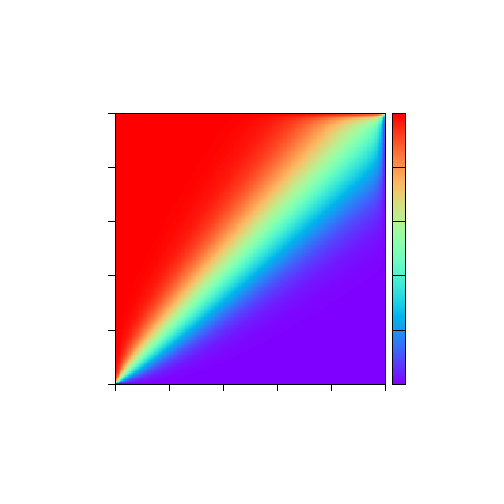
\includegraphics[width={226.70bp},height={226.70bp}]{figures/case_diagonal_flow/diagonal_N200_Pe1.0e+02}}%
    \gplfronttext
  \end{picture}%
\endgroup
}
		% GNUPLOT: LaTeX picture with Postscript
\begingroup
  % Encoding inside the plot.  In the header of your document, this encoding
  % should to defined, e.g., by using
  % \usepackage[cp1252,<other encodings>]{inputenc}
  \inputencoding{cp1252}%
  \makeatletter
  \providecommand\color[2][]{%
    \GenericError{(gnuplot) \space\space\space\@spaces}{%
      Package color not loaded in conjunction with
      terminal option `colourtext'%
    }{See the gnuplot documentation for explanation.%
    }{Either use 'blacktext' in gnuplot or load the package
      color.sty in LaTeX.}%
    \renewcommand\color[2][]{}%
  }%
  \providecommand\includegraphics[2][]{%
    \GenericError{(gnuplot) \space\space\space\@spaces}{%
      Package graphicx or graphics not loaded%
    }{See the gnuplot documentation for explanation.%
    }{The gnuplot epslatex terminal needs graphicx.sty or graphics.sty.}%
    \renewcommand\includegraphics[2][]{}%
  }%
  \providecommand\rotatebox[2]{#2}%
  \@ifundefined{ifGPcolor}{%
    \newif\ifGPcolor
    \GPcolortrue
  }{}%
  \@ifundefined{ifGPblacktext}{%
    \newif\ifGPblacktext
    \GPblacktextfalse
  }{}%
  % define a \g@addto@macro without @ in the name:
  \let\gplgaddtomacro\g@addto@macro
  % define empty templates for all commands taking text:
  \gdef\gplbacktext{}%
  \gdef\gplfronttext{}%
  \makeatother
  \ifGPblacktext
    % no textcolor at all
    \def\colorrgb#1{}%
    \def\colorgray#1{}%
  \else
    % gray or color?
    \ifGPcolor
      \def\colorrgb#1{\color[rgb]{#1}}%
      \def\colorgray#1{\color[gray]{#1}}%
      \expandafter\def\csname LTw\endcsname{\color{white}}%
      \expandafter\def\csname LTb\endcsname{\color{black}}%
      \expandafter\def\csname LTa\endcsname{\color{black}}%
      \expandafter\def\csname LT0\endcsname{\color[rgb]{1,0,0}}%
      \expandafter\def\csname LT1\endcsname{\color[rgb]{0,1,0}}%
      \expandafter\def\csname LT2\endcsname{\color[rgb]{0,0,1}}%
      \expandafter\def\csname LT3\endcsname{\color[rgb]{1,0,1}}%
      \expandafter\def\csname LT4\endcsname{\color[rgb]{0,1,1}}%
      \expandafter\def\csname LT5\endcsname{\color[rgb]{1,1,0}}%
      \expandafter\def\csname LT6\endcsname{\color[rgb]{0,0,0}}%
      \expandafter\def\csname LT7\endcsname{\color[rgb]{1,0.3,0}}%
      \expandafter\def\csname LT8\endcsname{\color[rgb]{0.5,0.5,0.5}}%
    \else
      % gray
      \def\colorrgb#1{\color{black}}%
      \def\colorgray#1{\color[gray]{#1}}%
      \expandafter\def\csname LTw\endcsname{\color{white}}%
      \expandafter\def\csname LTb\endcsname{\color{black}}%
      \expandafter\def\csname LTa\endcsname{\color{black}}%
      \expandafter\def\csname LT0\endcsname{\color{black}}%
      \expandafter\def\csname LT1\endcsname{\color{black}}%
      \expandafter\def\csname LT2\endcsname{\color{black}}%
      \expandafter\def\csname LT3\endcsname{\color{black}}%
      \expandafter\def\csname LT4\endcsname{\color{black}}%
      \expandafter\def\csname LT5\endcsname{\color{black}}%
      \expandafter\def\csname LT6\endcsname{\color{black}}%
      \expandafter\def\csname LT7\endcsname{\color{black}}%
      \expandafter\def\csname LT8\endcsname{\color{black}}%
    \fi
  \fi
    \setlength{\unitlength}{0.0500bp}%
    \ifx\gptboxheight\undefined%
      \newlength{\gptboxheight}%
      \newlength{\gptboxwidth}%
      \newsavebox{\gptboxtext}%
    \fi%
    \setlength{\fboxrule}{0.5pt}%
    \setlength{\fboxsep}{1pt}%
    \definecolor{tbcol}{rgb}{1,1,1}%
\begin{picture}(4534.00,4534.00)%
    \gplgaddtomacro\gplbacktext{%
      \csname LTb\endcsname%%
      \put(814,991){\makebox(0,0)[r]{\strut{}0.0}}%
      \put(814,1510){\makebox(0,0)[r]{\strut{}0.2}}%
      \put(814,2029){\makebox(0,0)[r]{\strut{}0.4}}%
      \put(814,2548){\makebox(0,0)[r]{\strut{}0.6}}%
      \put(814,3067){\makebox(0,0)[r]{\strut{}0.8}}%
      \put(814,3586){\makebox(0,0)[r]{\strut{}1.0}}%
      \put(946,771){\makebox(0,0){\strut{}0.0}}%
      \put(1465,771){\makebox(0,0){\strut{}0.2}}%
      \put(1984,771){\makebox(0,0){\strut{}0.4}}%
      \put(2502,771){\makebox(0,0){\strut{}0.6}}%
      \put(3021,771){\makebox(0,0){\strut{}0.8}}%
      \put(3540,771){\makebox(0,0){\strut{}1.0}}%
    }%
    \gplgaddtomacro\gplfronttext{%
      \csname LTb\endcsname%%
      \put(209,2288){\rotatebox{-270}{\makebox(0,0){\strut{}$y \ (\mathrm{m})$}}}%
      \put(2243,441){\makebox(0,0){\strut{}$x \ (\mathrm{m})$}}%
      \csname LTb\endcsname%%
      \put(3866,991){\makebox(0,0)[l]{\strut{}0.0}}%
      \put(3866,1510){\makebox(0,0)[l]{\strut{}0.2}}%
      \put(3866,2029){\makebox(0,0)[l]{\strut{}0.4}}%
      \put(3866,2548){\makebox(0,0)[l]{\strut{}0.6}}%
      \put(3866,3067){\makebox(0,0)[l]{\strut{}0.8}}%
      \put(3866,3586){\makebox(0,0)[l]{\strut{}1.0}}%
      \put(4328,2288){\rotatebox{-270}{\makebox(0,0){\strut{}$\phi$}}}%
      \put(2243,3916){\makebox(0,0){\strut{}\textbf{Diagonal case} $(\mathrm{Pe} = 10^{2})$}}%
    }%
    \gplbacktext
    \put(0,0){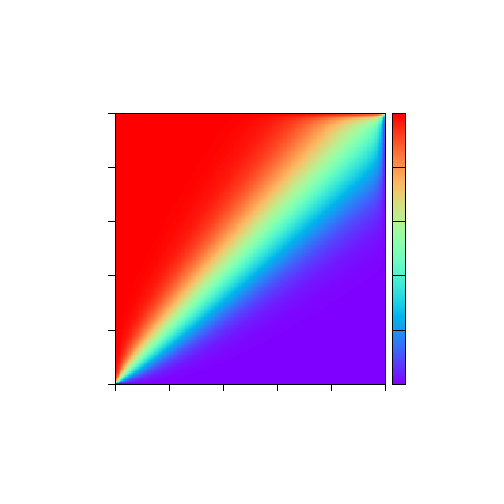
\includegraphics[width={226.70bp},height={226.70bp}]{figures/case_diagonal_flow/diagonal_N200_Pe1.0e+02}}%
    \gplfronttext
  \end{picture}%
\endgroup

		\vspace{-0.50cm}
		\captionsetup{width=0.8\textwidth}
		\caption{Numerical solution to the diagonal case for $\peclet = 10^2$.}
		\label{fig:diagonal_N200_Pe1.0e+02}
	\end{subfigure}
	\begin{subfigure}{.5\textwidth}
		\centering
		\vspace{-0.25cm}
%		\fbox{% GNUPLOT: LaTeX picture with Postscript
\begingroup
  % Encoding inside the plot.  In the header of your document, this encoding
  % should to defined, e.g., by using
  % \usepackage[cp1252,<other encodings>]{inputenc}
  \inputencoding{cp1252}%
  \makeatletter
  \providecommand\color[2][]{%
    \GenericError{(gnuplot) \space\space\space\@spaces}{%
      Package color not loaded in conjunction with
      terminal option `colourtext'%
    }{See the gnuplot documentation for explanation.%
    }{Either use 'blacktext' in gnuplot or load the package
      color.sty in LaTeX.}%
    \renewcommand\color[2][]{}%
  }%
  \providecommand\includegraphics[2][]{%
    \GenericError{(gnuplot) \space\space\space\@spaces}{%
      Package graphicx or graphics not loaded%
    }{See the gnuplot documentation for explanation.%
    }{The gnuplot epslatex terminal needs graphicx.sty or graphics.sty.}%
    \renewcommand\includegraphics[2][]{}%
  }%
  \providecommand\rotatebox[2]{#2}%
  \@ifundefined{ifGPcolor}{%
    \newif\ifGPcolor
    \GPcolortrue
  }{}%
  \@ifundefined{ifGPblacktext}{%
    \newif\ifGPblacktext
    \GPblacktextfalse
  }{}%
  % define a \g@addto@macro without @ in the name:
  \let\gplgaddtomacro\g@addto@macro
  % define empty templates for all commands taking text:
  \gdef\gplbacktext{}%
  \gdef\gplfronttext{}%
  \makeatother
  \ifGPblacktext
    % no textcolor at all
    \def\colorrgb#1{}%
    \def\colorgray#1{}%
  \else
    % gray or color?
    \ifGPcolor
      \def\colorrgb#1{\color[rgb]{#1}}%
      \def\colorgray#1{\color[gray]{#1}}%
      \expandafter\def\csname LTw\endcsname{\color{white}}%
      \expandafter\def\csname LTb\endcsname{\color{black}}%
      \expandafter\def\csname LTa\endcsname{\color{black}}%
      \expandafter\def\csname LT0\endcsname{\color[rgb]{1,0,0}}%
      \expandafter\def\csname LT1\endcsname{\color[rgb]{0,1,0}}%
      \expandafter\def\csname LT2\endcsname{\color[rgb]{0,0,1}}%
      \expandafter\def\csname LT3\endcsname{\color[rgb]{1,0,1}}%
      \expandafter\def\csname LT4\endcsname{\color[rgb]{0,1,1}}%
      \expandafter\def\csname LT5\endcsname{\color[rgb]{1,1,0}}%
      \expandafter\def\csname LT6\endcsname{\color[rgb]{0,0,0}}%
      \expandafter\def\csname LT7\endcsname{\color[rgb]{1,0.3,0}}%
      \expandafter\def\csname LT8\endcsname{\color[rgb]{0.5,0.5,0.5}}%
    \else
      % gray
      \def\colorrgb#1{\color{black}}%
      \def\colorgray#1{\color[gray]{#1}}%
      \expandafter\def\csname LTw\endcsname{\color{white}}%
      \expandafter\def\csname LTb\endcsname{\color{black}}%
      \expandafter\def\csname LTa\endcsname{\color{black}}%
      \expandafter\def\csname LT0\endcsname{\color{black}}%
      \expandafter\def\csname LT1\endcsname{\color{black}}%
      \expandafter\def\csname LT2\endcsname{\color{black}}%
      \expandafter\def\csname LT3\endcsname{\color{black}}%
      \expandafter\def\csname LT4\endcsname{\color{black}}%
      \expandafter\def\csname LT5\endcsname{\color{black}}%
      \expandafter\def\csname LT6\endcsname{\color{black}}%
      \expandafter\def\csname LT7\endcsname{\color{black}}%
      \expandafter\def\csname LT8\endcsname{\color{black}}%
    \fi
  \fi
    \setlength{\unitlength}{0.0500bp}%
    \ifx\gptboxheight\undefined%
      \newlength{\gptboxheight}%
      \newlength{\gptboxwidth}%
      \newsavebox{\gptboxtext}%
    \fi%
    \setlength{\fboxrule}{0.5pt}%
    \setlength{\fboxsep}{1pt}%
    \definecolor{tbcol}{rgb}{1,1,1}%
\begin{picture}(4534.00,4534.00)%
    \gplgaddtomacro\gplbacktext{%
      \csname LTb\endcsname%%
      \put(814,991){\makebox(0,0)[r]{\strut{}0.0}}%
      \put(814,1510){\makebox(0,0)[r]{\strut{}0.2}}%
      \put(814,2029){\makebox(0,0)[r]{\strut{}0.4}}%
      \put(814,2548){\makebox(0,0)[r]{\strut{}0.6}}%
      \put(814,3067){\makebox(0,0)[r]{\strut{}0.8}}%
      \put(814,3586){\makebox(0,0)[r]{\strut{}1.0}}%
      \put(946,771){\makebox(0,0){\strut{}0.0}}%
      \put(1465,771){\makebox(0,0){\strut{}0.2}}%
      \put(1984,771){\makebox(0,0){\strut{}0.4}}%
      \put(2502,771){\makebox(0,0){\strut{}0.6}}%
      \put(3021,771){\makebox(0,0){\strut{}0.8}}%
      \put(3540,771){\makebox(0,0){\strut{}1.0}}%
    }%
    \gplgaddtomacro\gplfronttext{%
      \csname LTb\endcsname%%
      \put(209,2288){\rotatebox{-270}{\makebox(0,0){\strut{}$y \ (\mathrm{m})$}}}%
      \put(2243,441){\makebox(0,0){\strut{}$x \ (\mathrm{m})$}}%
      \csname LTb\endcsname%%
      \put(3866,991){\makebox(0,0)[l]{\strut{}0.0}}%
      \put(3866,1510){\makebox(0,0)[l]{\strut{}0.2}}%
      \put(3866,2029){\makebox(0,0)[l]{\strut{}0.4}}%
      \put(3866,2548){\makebox(0,0)[l]{\strut{}0.6}}%
      \put(3866,3067){\makebox(0,0)[l]{\strut{}0.8}}%
      \put(3866,3586){\makebox(0,0)[l]{\strut{}1.0}}%
      \put(4328,2288){\rotatebox{-270}{\makebox(0,0){\strut{}$\phi$}}}%
      \put(2243,3916){\makebox(0,0){\strut{}\textbf{Diagonal case} $(\mathrm{Pe} = 10^{4})$}}%
    }%
    \gplbacktext
    \put(0,0){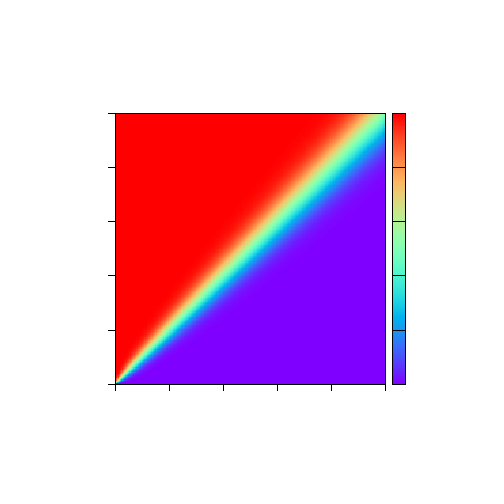
\includegraphics[width={226.70bp},height={226.70bp}]{figures/case_diagonal_flow/diagonal_N200_Pe1.0e+04}}%
    \gplfronttext
  \end{picture}%
\endgroup
}
		% GNUPLOT: LaTeX picture with Postscript
\begingroup
  % Encoding inside the plot.  In the header of your document, this encoding
  % should to defined, e.g., by using
  % \usepackage[cp1252,<other encodings>]{inputenc}
  \inputencoding{cp1252}%
  \makeatletter
  \providecommand\color[2][]{%
    \GenericError{(gnuplot) \space\space\space\@spaces}{%
      Package color not loaded in conjunction with
      terminal option `colourtext'%
    }{See the gnuplot documentation for explanation.%
    }{Either use 'blacktext' in gnuplot or load the package
      color.sty in LaTeX.}%
    \renewcommand\color[2][]{}%
  }%
  \providecommand\includegraphics[2][]{%
    \GenericError{(gnuplot) \space\space\space\@spaces}{%
      Package graphicx or graphics not loaded%
    }{See the gnuplot documentation for explanation.%
    }{The gnuplot epslatex terminal needs graphicx.sty or graphics.sty.}%
    \renewcommand\includegraphics[2][]{}%
  }%
  \providecommand\rotatebox[2]{#2}%
  \@ifundefined{ifGPcolor}{%
    \newif\ifGPcolor
    \GPcolortrue
  }{}%
  \@ifundefined{ifGPblacktext}{%
    \newif\ifGPblacktext
    \GPblacktextfalse
  }{}%
  % define a \g@addto@macro without @ in the name:
  \let\gplgaddtomacro\g@addto@macro
  % define empty templates for all commands taking text:
  \gdef\gplbacktext{}%
  \gdef\gplfronttext{}%
  \makeatother
  \ifGPblacktext
    % no textcolor at all
    \def\colorrgb#1{}%
    \def\colorgray#1{}%
  \else
    % gray or color?
    \ifGPcolor
      \def\colorrgb#1{\color[rgb]{#1}}%
      \def\colorgray#1{\color[gray]{#1}}%
      \expandafter\def\csname LTw\endcsname{\color{white}}%
      \expandafter\def\csname LTb\endcsname{\color{black}}%
      \expandafter\def\csname LTa\endcsname{\color{black}}%
      \expandafter\def\csname LT0\endcsname{\color[rgb]{1,0,0}}%
      \expandafter\def\csname LT1\endcsname{\color[rgb]{0,1,0}}%
      \expandafter\def\csname LT2\endcsname{\color[rgb]{0,0,1}}%
      \expandafter\def\csname LT3\endcsname{\color[rgb]{1,0,1}}%
      \expandafter\def\csname LT4\endcsname{\color[rgb]{0,1,1}}%
      \expandafter\def\csname LT5\endcsname{\color[rgb]{1,1,0}}%
      \expandafter\def\csname LT6\endcsname{\color[rgb]{0,0,0}}%
      \expandafter\def\csname LT7\endcsname{\color[rgb]{1,0.3,0}}%
      \expandafter\def\csname LT8\endcsname{\color[rgb]{0.5,0.5,0.5}}%
    \else
      % gray
      \def\colorrgb#1{\color{black}}%
      \def\colorgray#1{\color[gray]{#1}}%
      \expandafter\def\csname LTw\endcsname{\color{white}}%
      \expandafter\def\csname LTb\endcsname{\color{black}}%
      \expandafter\def\csname LTa\endcsname{\color{black}}%
      \expandafter\def\csname LT0\endcsname{\color{black}}%
      \expandafter\def\csname LT1\endcsname{\color{black}}%
      \expandafter\def\csname LT2\endcsname{\color{black}}%
      \expandafter\def\csname LT3\endcsname{\color{black}}%
      \expandafter\def\csname LT4\endcsname{\color{black}}%
      \expandafter\def\csname LT5\endcsname{\color{black}}%
      \expandafter\def\csname LT6\endcsname{\color{black}}%
      \expandafter\def\csname LT7\endcsname{\color{black}}%
      \expandafter\def\csname LT8\endcsname{\color{black}}%
    \fi
  \fi
    \setlength{\unitlength}{0.0500bp}%
    \ifx\gptboxheight\undefined%
      \newlength{\gptboxheight}%
      \newlength{\gptboxwidth}%
      \newsavebox{\gptboxtext}%
    \fi%
    \setlength{\fboxrule}{0.5pt}%
    \setlength{\fboxsep}{1pt}%
    \definecolor{tbcol}{rgb}{1,1,1}%
\begin{picture}(4534.00,4534.00)%
    \gplgaddtomacro\gplbacktext{%
      \csname LTb\endcsname%%
      \put(814,991){\makebox(0,0)[r]{\strut{}0.0}}%
      \put(814,1510){\makebox(0,0)[r]{\strut{}0.2}}%
      \put(814,2029){\makebox(0,0)[r]{\strut{}0.4}}%
      \put(814,2548){\makebox(0,0)[r]{\strut{}0.6}}%
      \put(814,3067){\makebox(0,0)[r]{\strut{}0.8}}%
      \put(814,3586){\makebox(0,0)[r]{\strut{}1.0}}%
      \put(946,771){\makebox(0,0){\strut{}0.0}}%
      \put(1465,771){\makebox(0,0){\strut{}0.2}}%
      \put(1984,771){\makebox(0,0){\strut{}0.4}}%
      \put(2502,771){\makebox(0,0){\strut{}0.6}}%
      \put(3021,771){\makebox(0,0){\strut{}0.8}}%
      \put(3540,771){\makebox(0,0){\strut{}1.0}}%
    }%
    \gplgaddtomacro\gplfronttext{%
      \csname LTb\endcsname%%
      \put(209,2288){\rotatebox{-270}{\makebox(0,0){\strut{}$y \ (\mathrm{m})$}}}%
      \put(2243,441){\makebox(0,0){\strut{}$x \ (\mathrm{m})$}}%
      \csname LTb\endcsname%%
      \put(3866,991){\makebox(0,0)[l]{\strut{}0.0}}%
      \put(3866,1510){\makebox(0,0)[l]{\strut{}0.2}}%
      \put(3866,2029){\makebox(0,0)[l]{\strut{}0.4}}%
      \put(3866,2548){\makebox(0,0)[l]{\strut{}0.6}}%
      \put(3866,3067){\makebox(0,0)[l]{\strut{}0.8}}%
      \put(3866,3586){\makebox(0,0)[l]{\strut{}1.0}}%
      \put(4328,2288){\rotatebox{-270}{\makebox(0,0){\strut{}$\phi$}}}%
      \put(2243,3916){\makebox(0,0){\strut{}\textbf{Diagonal case} $(\mathrm{Pe} = 10^{4})$}}%
    }%
    \gplbacktext
    \put(0,0){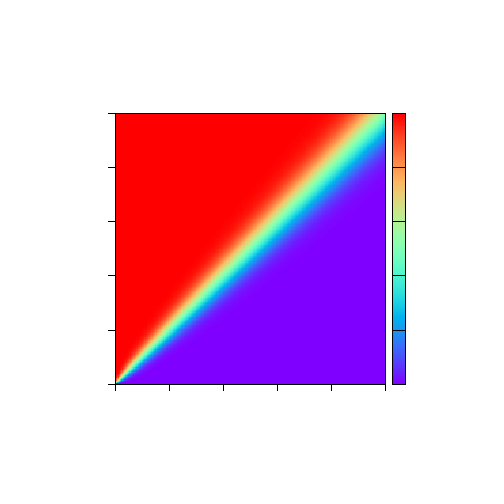
\includegraphics[width={226.70bp},height={226.70bp}]{figures/case_diagonal_flow/diagonal_N200_Pe1.0e+04}}%
    \gplfronttext
  \end{picture}%
\endgroup

		\vspace{-0.50cm}
		\captionsetup{width=0.8\textwidth}
		\caption{Numerical solution to the diagonal case for $\peclet = 10^3$.}
		\label{fig:diagonal_N200_Pe1.0e+04}
	\end{subfigure}%
	\begin{subfigure}{.5\textwidth}
		\centering
		\vspace{-0.25cm}
		%		\fbox{% GNUPLOT: LaTeX picture with Postscript
\begingroup
  % Encoding inside the plot.  In the header of your document, this encoding
  % should to defined, e.g., by using
  % \usepackage[cp1252,<other encodings>]{inputenc}
  \inputencoding{cp1252}%
  \makeatletter
  \providecommand\color[2][]{%
    \GenericError{(gnuplot) \space\space\space\@spaces}{%
      Package color not loaded in conjunction with
      terminal option `colourtext'%
    }{See the gnuplot documentation for explanation.%
    }{Either use 'blacktext' in gnuplot or load the package
      color.sty in LaTeX.}%
    \renewcommand\color[2][]{}%
  }%
  \providecommand\includegraphics[2][]{%
    \GenericError{(gnuplot) \space\space\space\@spaces}{%
      Package graphicx or graphics not loaded%
    }{See the gnuplot documentation for explanation.%
    }{The gnuplot epslatex terminal needs graphicx.sty or graphics.sty.}%
    \renewcommand\includegraphics[2][]{}%
  }%
  \providecommand\rotatebox[2]{#2}%
  \@ifundefined{ifGPcolor}{%
    \newif\ifGPcolor
    \GPcolortrue
  }{}%
  \@ifundefined{ifGPblacktext}{%
    \newif\ifGPblacktext
    \GPblacktextfalse
  }{}%
  % define a \g@addto@macro without @ in the name:
  \let\gplgaddtomacro\g@addto@macro
  % define empty templates for all commands taking text:
  \gdef\gplbacktext{}%
  \gdef\gplfronttext{}%
  \makeatother
  \ifGPblacktext
    % no textcolor at all
    \def\colorrgb#1{}%
    \def\colorgray#1{}%
  \else
    % gray or color?
    \ifGPcolor
      \def\colorrgb#1{\color[rgb]{#1}}%
      \def\colorgray#1{\color[gray]{#1}}%
      \expandafter\def\csname LTw\endcsname{\color{white}}%
      \expandafter\def\csname LTb\endcsname{\color{black}}%
      \expandafter\def\csname LTa\endcsname{\color{black}}%
      \expandafter\def\csname LT0\endcsname{\color[rgb]{1,0,0}}%
      \expandafter\def\csname LT1\endcsname{\color[rgb]{0,1,0}}%
      \expandafter\def\csname LT2\endcsname{\color[rgb]{0,0,1}}%
      \expandafter\def\csname LT3\endcsname{\color[rgb]{1,0,1}}%
      \expandafter\def\csname LT4\endcsname{\color[rgb]{0,1,1}}%
      \expandafter\def\csname LT5\endcsname{\color[rgb]{1,1,0}}%
      \expandafter\def\csname LT6\endcsname{\color[rgb]{0,0,0}}%
      \expandafter\def\csname LT7\endcsname{\color[rgb]{1,0.3,0}}%
      \expandafter\def\csname LT8\endcsname{\color[rgb]{0.5,0.5,0.5}}%
    \else
      % gray
      \def\colorrgb#1{\color{black}}%
      \def\colorgray#1{\color[gray]{#1}}%
      \expandafter\def\csname LTw\endcsname{\color{white}}%
      \expandafter\def\csname LTb\endcsname{\color{black}}%
      \expandafter\def\csname LTa\endcsname{\color{black}}%
      \expandafter\def\csname LT0\endcsname{\color{black}}%
      \expandafter\def\csname LT1\endcsname{\color{black}}%
      \expandafter\def\csname LT2\endcsname{\color{black}}%
      \expandafter\def\csname LT3\endcsname{\color{black}}%
      \expandafter\def\csname LT4\endcsname{\color{black}}%
      \expandafter\def\csname LT5\endcsname{\color{black}}%
      \expandafter\def\csname LT6\endcsname{\color{black}}%
      \expandafter\def\csname LT7\endcsname{\color{black}}%
      \expandafter\def\csname LT8\endcsname{\color{black}}%
    \fi
  \fi
    \setlength{\unitlength}{0.0500bp}%
    \ifx\gptboxheight\undefined%
      \newlength{\gptboxheight}%
      \newlength{\gptboxwidth}%
      \newsavebox{\gptboxtext}%
    \fi%
    \setlength{\fboxrule}{0.5pt}%
    \setlength{\fboxsep}{1pt}%
    \definecolor{tbcol}{rgb}{1,1,1}%
\begin{picture}(4534.00,4534.00)%
    \gplgaddtomacro\gplbacktext{%
      \csname LTb\endcsname%%
      \put(814,991){\makebox(0,0)[r]{\strut{}0.0}}%
      \put(814,1510){\makebox(0,0)[r]{\strut{}0.2}}%
      \put(814,2029){\makebox(0,0)[r]{\strut{}0.4}}%
      \put(814,2548){\makebox(0,0)[r]{\strut{}0.6}}%
      \put(814,3067){\makebox(0,0)[r]{\strut{}0.8}}%
      \put(814,3586){\makebox(0,0)[r]{\strut{}1.0}}%
      \put(946,771){\makebox(0,0){\strut{}0.0}}%
      \put(1465,771){\makebox(0,0){\strut{}0.2}}%
      \put(1984,771){\makebox(0,0){\strut{}0.4}}%
      \put(2502,771){\makebox(0,0){\strut{}0.6}}%
      \put(3021,771){\makebox(0,0){\strut{}0.8}}%
      \put(3540,771){\makebox(0,0){\strut{}1.0}}%
    }%
    \gplgaddtomacro\gplfronttext{%
      \csname LTb\endcsname%%
      \put(209,2288){\rotatebox{-270}{\makebox(0,0){\strut{}$y \ (\mathrm{m})$}}}%
      \put(2243,441){\makebox(0,0){\strut{}$x \ (\mathrm{m})$}}%
      \csname LTb\endcsname%%
      \put(3866,991){\makebox(0,0)[l]{\strut{}0.0}}%
      \put(3866,1510){\makebox(0,0)[l]{\strut{}0.2}}%
      \put(3866,2029){\makebox(0,0)[l]{\strut{}0.4}}%
      \put(3866,2548){\makebox(0,0)[l]{\strut{}0.6}}%
      \put(3866,3067){\makebox(0,0)[l]{\strut{}0.8}}%
      \put(3866,3586){\makebox(0,0)[l]{\strut{}1.0}}%
      \put(4328,2288){\rotatebox{-270}{\makebox(0,0){\strut{}$\phi$}}}%
      \put(2243,3916){\makebox(0,0){\strut{}\textbf{Diagonal flow} $(\mathrm{Pe} = 10^{9})$}}%
    }%
    \gplbacktext
    \put(0,0){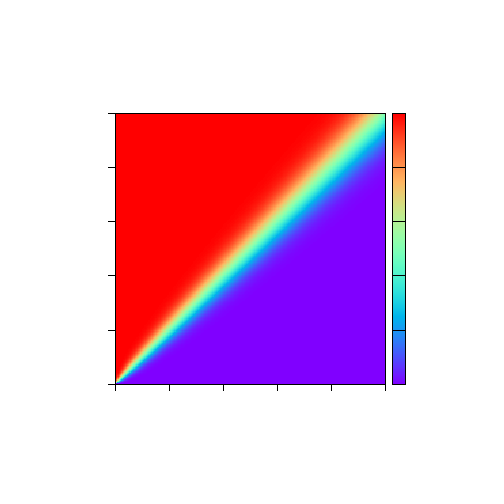
\includegraphics[width={226.70bp},height={226.70bp}]{figures/case_diagonal_flow/diagonal_N200_Pe1.0e+09}}%
    \gplfronttext
  \end{picture}%
\endgroup
}
		% GNUPLOT: LaTeX picture with Postscript
\begingroup
  % Encoding inside the plot.  In the header of your document, this encoding
  % should to defined, e.g., by using
  % \usepackage[cp1252,<other encodings>]{inputenc}
  \inputencoding{cp1252}%
  \makeatletter
  \providecommand\color[2][]{%
    \GenericError{(gnuplot) \space\space\space\@spaces}{%
      Package color not loaded in conjunction with
      terminal option `colourtext'%
    }{See the gnuplot documentation for explanation.%
    }{Either use 'blacktext' in gnuplot or load the package
      color.sty in LaTeX.}%
    \renewcommand\color[2][]{}%
  }%
  \providecommand\includegraphics[2][]{%
    \GenericError{(gnuplot) \space\space\space\@spaces}{%
      Package graphicx or graphics not loaded%
    }{See the gnuplot documentation for explanation.%
    }{The gnuplot epslatex terminal needs graphicx.sty or graphics.sty.}%
    \renewcommand\includegraphics[2][]{}%
  }%
  \providecommand\rotatebox[2]{#2}%
  \@ifundefined{ifGPcolor}{%
    \newif\ifGPcolor
    \GPcolortrue
  }{}%
  \@ifundefined{ifGPblacktext}{%
    \newif\ifGPblacktext
    \GPblacktextfalse
  }{}%
  % define a \g@addto@macro without @ in the name:
  \let\gplgaddtomacro\g@addto@macro
  % define empty templates for all commands taking text:
  \gdef\gplbacktext{}%
  \gdef\gplfronttext{}%
  \makeatother
  \ifGPblacktext
    % no textcolor at all
    \def\colorrgb#1{}%
    \def\colorgray#1{}%
  \else
    % gray or color?
    \ifGPcolor
      \def\colorrgb#1{\color[rgb]{#1}}%
      \def\colorgray#1{\color[gray]{#1}}%
      \expandafter\def\csname LTw\endcsname{\color{white}}%
      \expandafter\def\csname LTb\endcsname{\color{black}}%
      \expandafter\def\csname LTa\endcsname{\color{black}}%
      \expandafter\def\csname LT0\endcsname{\color[rgb]{1,0,0}}%
      \expandafter\def\csname LT1\endcsname{\color[rgb]{0,1,0}}%
      \expandafter\def\csname LT2\endcsname{\color[rgb]{0,0,1}}%
      \expandafter\def\csname LT3\endcsname{\color[rgb]{1,0,1}}%
      \expandafter\def\csname LT4\endcsname{\color[rgb]{0,1,1}}%
      \expandafter\def\csname LT5\endcsname{\color[rgb]{1,1,0}}%
      \expandafter\def\csname LT6\endcsname{\color[rgb]{0,0,0}}%
      \expandafter\def\csname LT7\endcsname{\color[rgb]{1,0.3,0}}%
      \expandafter\def\csname LT8\endcsname{\color[rgb]{0.5,0.5,0.5}}%
    \else
      % gray
      \def\colorrgb#1{\color{black}}%
      \def\colorgray#1{\color[gray]{#1}}%
      \expandafter\def\csname LTw\endcsname{\color{white}}%
      \expandafter\def\csname LTb\endcsname{\color{black}}%
      \expandafter\def\csname LTa\endcsname{\color{black}}%
      \expandafter\def\csname LT0\endcsname{\color{black}}%
      \expandafter\def\csname LT1\endcsname{\color{black}}%
      \expandafter\def\csname LT2\endcsname{\color{black}}%
      \expandafter\def\csname LT3\endcsname{\color{black}}%
      \expandafter\def\csname LT4\endcsname{\color{black}}%
      \expandafter\def\csname LT5\endcsname{\color{black}}%
      \expandafter\def\csname LT6\endcsname{\color{black}}%
      \expandafter\def\csname LT7\endcsname{\color{black}}%
      \expandafter\def\csname LT8\endcsname{\color{black}}%
    \fi
  \fi
    \setlength{\unitlength}{0.0500bp}%
    \ifx\gptboxheight\undefined%
      \newlength{\gptboxheight}%
      \newlength{\gptboxwidth}%
      \newsavebox{\gptboxtext}%
    \fi%
    \setlength{\fboxrule}{0.5pt}%
    \setlength{\fboxsep}{1pt}%
    \definecolor{tbcol}{rgb}{1,1,1}%
\begin{picture}(4534.00,4534.00)%
    \gplgaddtomacro\gplbacktext{%
      \csname LTb\endcsname%%
      \put(814,991){\makebox(0,0)[r]{\strut{}0.0}}%
      \put(814,1510){\makebox(0,0)[r]{\strut{}0.2}}%
      \put(814,2029){\makebox(0,0)[r]{\strut{}0.4}}%
      \put(814,2548){\makebox(0,0)[r]{\strut{}0.6}}%
      \put(814,3067){\makebox(0,0)[r]{\strut{}0.8}}%
      \put(814,3586){\makebox(0,0)[r]{\strut{}1.0}}%
      \put(946,771){\makebox(0,0){\strut{}0.0}}%
      \put(1465,771){\makebox(0,0){\strut{}0.2}}%
      \put(1984,771){\makebox(0,0){\strut{}0.4}}%
      \put(2502,771){\makebox(0,0){\strut{}0.6}}%
      \put(3021,771){\makebox(0,0){\strut{}0.8}}%
      \put(3540,771){\makebox(0,0){\strut{}1.0}}%
    }%
    \gplgaddtomacro\gplfronttext{%
      \csname LTb\endcsname%%
      \put(209,2288){\rotatebox{-270}{\makebox(0,0){\strut{}$y \ (\mathrm{m})$}}}%
      \put(2243,441){\makebox(0,0){\strut{}$x \ (\mathrm{m})$}}%
      \csname LTb\endcsname%%
      \put(3866,991){\makebox(0,0)[l]{\strut{}0.0}}%
      \put(3866,1510){\makebox(0,0)[l]{\strut{}0.2}}%
      \put(3866,2029){\makebox(0,0)[l]{\strut{}0.4}}%
      \put(3866,2548){\makebox(0,0)[l]{\strut{}0.6}}%
      \put(3866,3067){\makebox(0,0)[l]{\strut{}0.8}}%
      \put(3866,3586){\makebox(0,0)[l]{\strut{}1.0}}%
      \put(4328,2288){\rotatebox{-270}{\makebox(0,0){\strut{}$\phi$}}}%
      \put(2243,3916){\makebox(0,0){\strut{}\textbf{Diagonal flow} $(\mathrm{Pe} = 10^{9})$}}%
    }%
    \gplbacktext
    \put(0,0){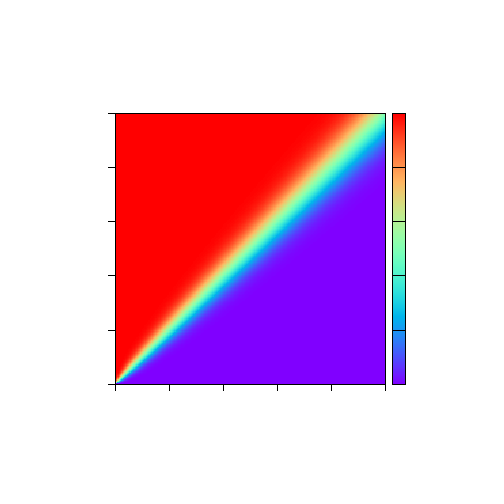
\includegraphics[width={226.70bp},height={226.70bp}]{figures/case_diagonal_flow/diagonal_N200_Pe1.0e+09}}%
    \gplfronttext
  \end{picture}%
\endgroup

		\vspace{-0.50cm}
		\captionsetup{width=0.8\textwidth}
		\caption{Numerical solution to the diagonal case for $\peclet = 1^90$.}
		\label{fig:diagonal_N200_Pe1.0e+09}
	\end{subfigure}%
	\caption{Numerical solution to the diagonal case for $\peclet = 10, \ 10^2, 10^4$ and $10^9$.}
	\label{fig:diagonal_N200_Pe_greater_than_1}
\end{figure}

\clearpage
Figures \ref{fig:diagonal_N200_Pe1.0e-01} to \ref{fig:diagonal_N200_Pe1.0e-09} show the diagonal case solution to $\peclet = 10^{-1}, \ 10^{-2}, \ 10^{-4}$ and $10^{-9}$. As it can be observed, all the solutions have a similar appearance to that for $\peclet = 1$ (figure \ref{fig:diagonal_N200_Pe1.0e+00}), whence it can be deduced that reducing Péclet's number has not obvious effect.

\begin{figure}[h]
	\centering
	\begin{subfigure}{.5\textwidth}
		\centering
		\vspace{-0.75cm}
		%		\fbox{% GNUPLOT: LaTeX picture with Postscript
\documentclass{minimal}
% Set font size
\makeatletter
\def\@ptsize{1}
\InputIfFileExists{size11.clo}{}{%
   \GenericError{(gnuplot) \space\space\space\@spaces}{%
      Gnuplot Error: File `size11.clo' not found! Could not set font size%
   }{See the gnuplot documentation for explanation.%
   }{For using a font size a file `size<fontsize>.clo' has to exist.
        Falling back ^^Jto default fontsize 10pt.}%
  \def\@ptsize{0}
  \input{size10.clo}%
}%
\makeatother
% Load packages
\usepackage{calc}
\usepackage{graphicx}
\usepackage{color}
\usepackage[cp1252]{inputenc}
\makeatletter
% Select an appropriate default driver (from TeXLive graphics.cfg)
\begingroup
  \chardef\x=0 %
  % check pdfTeX
  \@ifundefined{pdfoutput}{}{%
    \ifcase\pdfoutput
    \else
      \chardef\x=1 %
    \fi
  }%
  % check VTeX
  \@ifundefined{OpMode}{}{%
    \chardef\x=2 %
  }%
\expandafter\endgroup
\ifcase\x
  % default case
  \PassOptionsToPackage{dvips}{geometry}
\or
  % pdfTeX is running in pdf mode
  \PassOptionsToPackage{pdftex}{geometry}
\else
  % VTeX is running
  \PassOptionsToPackage{vtex}{geometry}
\fi
\makeatother
% Set papersize
\usepackage[papersize={340.10bp,340.10bp},text={340.10bp,340.10bp}]{geometry}
% No page numbers and no paragraph indentation
\pagestyle{empty}
\setlength{\parindent}{0bp}%
% Load configuration file
\InputIfFileExists{gnuplot.cfg}{%
  \typeout{Using configuration file gnuplot.cfg}%
}{%
 \typeout{No configuration file gnuplot.cfg found.}%
}%
%
\begin{document}
\begingroup
  % Encoding inside the plot.  In the header of your document, this encoding
  % should to defined, e.g., by using
  % \usepackage[cp1252,<other encodings>]{inputenc}
  \inputencoding{cp1252}%
  \makeatletter
  \providecommand\color[2][]{%
    \GenericError{(gnuplot) \space\space\space\@spaces}{%
      Package color not loaded in conjunction with
      terminal option `colourtext'%
    }{See the gnuplot documentation for explanation.%
    }{Either use 'blacktext' in gnuplot or load the package
      color.sty in LaTeX.}%
    \renewcommand\color[2][]{}%
  }%
  \providecommand\includegraphics[2][]{%
    \GenericError{(gnuplot) \space\space\space\@spaces}{%
      Package graphicx or graphics not loaded%
    }{See the gnuplot documentation for explanation.%
    }{The gnuplot epslatex terminal needs graphicx.sty or graphics.sty.}%
    \renewcommand\includegraphics[2][]{}%
  }%
  \providecommand\rotatebox[2]{#2}%
  \@ifundefined{ifGPcolor}{%
    \newif\ifGPcolor
    \GPcolortrue
  }{}%
  \@ifundefined{ifGPblacktext}{%
    \newif\ifGPblacktext
    \GPblacktextfalse
  }{}%
  % define a \g@addto@macro without @ in the name:
  \let\gplgaddtomacro\g@addto@macro
  % define empty templates for all commands taking text:
  \gdef\gplbacktext{}%
  \gdef\gplfronttext{}%
  \makeatother
  \ifGPblacktext
    % no textcolor at all
    \def\colorrgb#1{}%
    \def\colorgray#1{}%
  \else
    % gray or color?
    \ifGPcolor
      \def\colorrgb#1{\color[rgb]{#1}}%
      \def\colorgray#1{\color[gray]{#1}}%
      \expandafter\def\csname LTw\endcsname{\color{white}}%
      \expandafter\def\csname LTb\endcsname{\color{black}}%
      \expandafter\def\csname LTa\endcsname{\color{black}}%
      \expandafter\def\csname LT0\endcsname{\color[rgb]{1,0,0}}%
      \expandafter\def\csname LT1\endcsname{\color[rgb]{0,1,0}}%
      \expandafter\def\csname LT2\endcsname{\color[rgb]{0,0,1}}%
      \expandafter\def\csname LT3\endcsname{\color[rgb]{1,0,1}}%
      \expandafter\def\csname LT4\endcsname{\color[rgb]{0,1,1}}%
      \expandafter\def\csname LT5\endcsname{\color[rgb]{1,1,0}}%
      \expandafter\def\csname LT6\endcsname{\color[rgb]{0,0,0}}%
      \expandafter\def\csname LT7\endcsname{\color[rgb]{1,0.3,0}}%
      \expandafter\def\csname LT8\endcsname{\color[rgb]{0.5,0.5,0.5}}%
    \else
      % gray
      \def\colorrgb#1{\color{black}}%
      \def\colorgray#1{\color[gray]{#1}}%
      \expandafter\def\csname LTw\endcsname{\color{white}}%
      \expandafter\def\csname LTb\endcsname{\color{black}}%
      \expandafter\def\csname LTa\endcsname{\color{black}}%
      \expandafter\def\csname LT0\endcsname{\color{black}}%
      \expandafter\def\csname LT1\endcsname{\color{black}}%
      \expandafter\def\csname LT2\endcsname{\color{black}}%
      \expandafter\def\csname LT3\endcsname{\color{black}}%
      \expandafter\def\csname LT4\endcsname{\color{black}}%
      \expandafter\def\csname LT5\endcsname{\color{black}}%
      \expandafter\def\csname LT6\endcsname{\color{black}}%
      \expandafter\def\csname LT7\endcsname{\color{black}}%
      \expandafter\def\csname LT8\endcsname{\color{black}}%
    \fi
  \fi
    \setlength{\unitlength}{0.0500bp}%
    \ifx\gptboxheight\undefined%
      \newlength{\gptboxheight}%
      \newlength{\gptboxwidth}%
      \newsavebox{\gptboxtext}%
    \fi%
    \setlength{\fboxrule}{0.5pt}%
    \setlength{\fboxsep}{1pt}%
    \definecolor{tbcol}{rgb}{1,1,1}%
\begin{picture}(6802.00,6802.00)%
    \gplgaddtomacro\gplbacktext{%
      \csname LTb\endcsname%%
      \put(814,1105){\makebox(0,0)[r]{\strut{}0.0}}%
      \put(814,2032){\makebox(0,0)[r]{\strut{}0.2}}%
      \put(814,2959){\makebox(0,0)[r]{\strut{}0.4}}%
      \put(814,3886){\makebox(0,0)[r]{\strut{}0.6}}%
      \put(814,4813){\makebox(0,0)[r]{\strut{}0.8}}%
      \put(814,5740){\makebox(0,0)[r]{\strut{}1.0}}%
      \put(946,885){\makebox(0,0){\strut{}0.0}}%
      \put(1873,885){\makebox(0,0){\strut{}0.2}}%
      \put(2800,885){\makebox(0,0){\strut{}0.4}}%
      \put(3727,885){\makebox(0,0){\strut{}0.6}}%
      \put(4654,885){\makebox(0,0){\strut{}0.8}}%
      \put(5581,885){\makebox(0,0){\strut{}1.0}}%
    }%
    \gplgaddtomacro\gplfronttext{%
      \csname LTb\endcsname%%
      \put(209,3422){\rotatebox{-270}{\makebox(0,0){\strut{}$y \ (\mathrm{m})$}}}%
      \put(3263,555){\makebox(0,0){\strut{}$x \ (\mathrm{m})$}}%
      \csname LTb\endcsname%%
      \put(6060,1105){\makebox(0,0)[l]{\strut{}0.0}}%
      \put(6060,2032){\makebox(0,0)[l]{\strut{}0.2}}%
      \put(6060,2959){\makebox(0,0)[l]{\strut{}0.4}}%
      \put(6060,3886){\makebox(0,0)[l]{\strut{}0.6}}%
      \put(6060,4813){\makebox(0,0)[l]{\strut{}0.8}}%
      \put(6060,5740){\makebox(0,0)[l]{\strut{}1.0}}%
      \put(6522,3422){\rotatebox{-270}{\makebox(0,0){\strut{}$\phi$}}}%
      \put(3263,6070){\makebox(0,0){\strut{}\textbf{Diagonal case} $(\mathrm{Pe} = 10^{-1})$}}%
    }%
    \gplbacktext
    \put(0,0){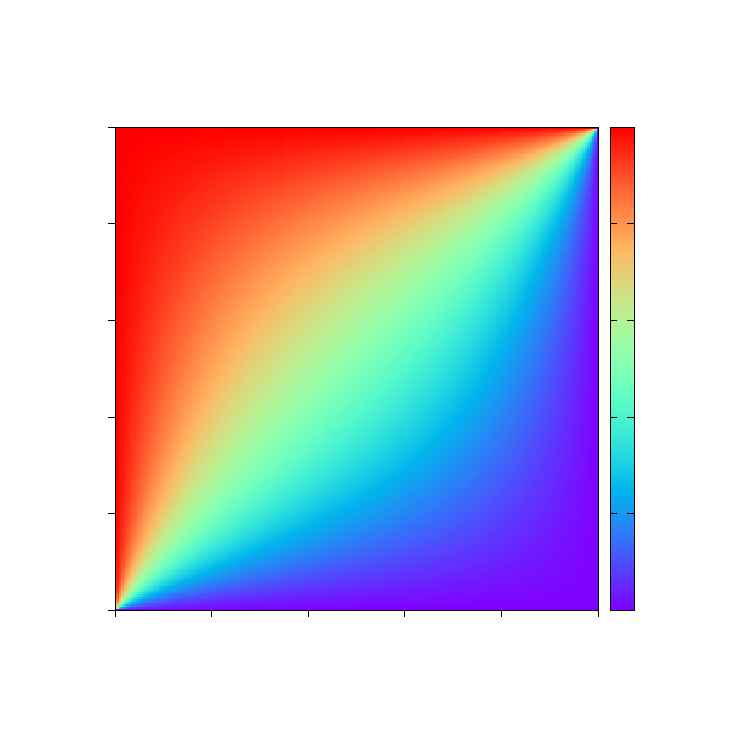
\includegraphics[width={340.10bp},height={340.10bp}]{standalone/case_diagonal_flow/diagonal_N200_Pe1.0e-01-inc}}%
    \gplfronttext
  \end{picture}%
\endgroup
\end{document}
}
		% GNUPLOT: LaTeX picture with Postscript
\documentclass{minimal}
% Set font size
\makeatletter
\def\@ptsize{1}
\InputIfFileExists{size11.clo}{}{%
   \GenericError{(gnuplot) \space\space\space\@spaces}{%
      Gnuplot Error: File `size11.clo' not found! Could not set font size%
   }{See the gnuplot documentation for explanation.%
   }{For using a font size a file `size<fontsize>.clo' has to exist.
        Falling back ^^Jto default fontsize 10pt.}%
  \def\@ptsize{0}
  \input{size10.clo}%
}%
\makeatother
% Load packages
\usepackage{calc}
\usepackage{graphicx}
\usepackage{color}
\usepackage[cp1252]{inputenc}
\makeatletter
% Select an appropriate default driver (from TeXLive graphics.cfg)
\begingroup
  \chardef\x=0 %
  % check pdfTeX
  \@ifundefined{pdfoutput}{}{%
    \ifcase\pdfoutput
    \else
      \chardef\x=1 %
    \fi
  }%
  % check VTeX
  \@ifundefined{OpMode}{}{%
    \chardef\x=2 %
  }%
\expandafter\endgroup
\ifcase\x
  % default case
  \PassOptionsToPackage{dvips}{geometry}
\or
  % pdfTeX is running in pdf mode
  \PassOptionsToPackage{pdftex}{geometry}
\else
  % VTeX is running
  \PassOptionsToPackage{vtex}{geometry}
\fi
\makeatother
% Set papersize
\usepackage[papersize={340.10bp,340.10bp},text={340.10bp,340.10bp}]{geometry}
% No page numbers and no paragraph indentation
\pagestyle{empty}
\setlength{\parindent}{0bp}%
% Load configuration file
\InputIfFileExists{gnuplot.cfg}{%
  \typeout{Using configuration file gnuplot.cfg}%
}{%
 \typeout{No configuration file gnuplot.cfg found.}%
}%
%
\begin{document}
\begingroup
  % Encoding inside the plot.  In the header of your document, this encoding
  % should to defined, e.g., by using
  % \usepackage[cp1252,<other encodings>]{inputenc}
  \inputencoding{cp1252}%
  \makeatletter
  \providecommand\color[2][]{%
    \GenericError{(gnuplot) \space\space\space\@spaces}{%
      Package color not loaded in conjunction with
      terminal option `colourtext'%
    }{See the gnuplot documentation for explanation.%
    }{Either use 'blacktext' in gnuplot or load the package
      color.sty in LaTeX.}%
    \renewcommand\color[2][]{}%
  }%
  \providecommand\includegraphics[2][]{%
    \GenericError{(gnuplot) \space\space\space\@spaces}{%
      Package graphicx or graphics not loaded%
    }{See the gnuplot documentation for explanation.%
    }{The gnuplot epslatex terminal needs graphicx.sty or graphics.sty.}%
    \renewcommand\includegraphics[2][]{}%
  }%
  \providecommand\rotatebox[2]{#2}%
  \@ifundefined{ifGPcolor}{%
    \newif\ifGPcolor
    \GPcolortrue
  }{}%
  \@ifundefined{ifGPblacktext}{%
    \newif\ifGPblacktext
    \GPblacktextfalse
  }{}%
  % define a \g@addto@macro without @ in the name:
  \let\gplgaddtomacro\g@addto@macro
  % define empty templates for all commands taking text:
  \gdef\gplbacktext{}%
  \gdef\gplfronttext{}%
  \makeatother
  \ifGPblacktext
    % no textcolor at all
    \def\colorrgb#1{}%
    \def\colorgray#1{}%
  \else
    % gray or color?
    \ifGPcolor
      \def\colorrgb#1{\color[rgb]{#1}}%
      \def\colorgray#1{\color[gray]{#1}}%
      \expandafter\def\csname LTw\endcsname{\color{white}}%
      \expandafter\def\csname LTb\endcsname{\color{black}}%
      \expandafter\def\csname LTa\endcsname{\color{black}}%
      \expandafter\def\csname LT0\endcsname{\color[rgb]{1,0,0}}%
      \expandafter\def\csname LT1\endcsname{\color[rgb]{0,1,0}}%
      \expandafter\def\csname LT2\endcsname{\color[rgb]{0,0,1}}%
      \expandafter\def\csname LT3\endcsname{\color[rgb]{1,0,1}}%
      \expandafter\def\csname LT4\endcsname{\color[rgb]{0,1,1}}%
      \expandafter\def\csname LT5\endcsname{\color[rgb]{1,1,0}}%
      \expandafter\def\csname LT6\endcsname{\color[rgb]{0,0,0}}%
      \expandafter\def\csname LT7\endcsname{\color[rgb]{1,0.3,0}}%
      \expandafter\def\csname LT8\endcsname{\color[rgb]{0.5,0.5,0.5}}%
    \else
      % gray
      \def\colorrgb#1{\color{black}}%
      \def\colorgray#1{\color[gray]{#1}}%
      \expandafter\def\csname LTw\endcsname{\color{white}}%
      \expandafter\def\csname LTb\endcsname{\color{black}}%
      \expandafter\def\csname LTa\endcsname{\color{black}}%
      \expandafter\def\csname LT0\endcsname{\color{black}}%
      \expandafter\def\csname LT1\endcsname{\color{black}}%
      \expandafter\def\csname LT2\endcsname{\color{black}}%
      \expandafter\def\csname LT3\endcsname{\color{black}}%
      \expandafter\def\csname LT4\endcsname{\color{black}}%
      \expandafter\def\csname LT5\endcsname{\color{black}}%
      \expandafter\def\csname LT6\endcsname{\color{black}}%
      \expandafter\def\csname LT7\endcsname{\color{black}}%
      \expandafter\def\csname LT8\endcsname{\color{black}}%
    \fi
  \fi
    \setlength{\unitlength}{0.0500bp}%
    \ifx\gptboxheight\undefined%
      \newlength{\gptboxheight}%
      \newlength{\gptboxwidth}%
      \newsavebox{\gptboxtext}%
    \fi%
    \setlength{\fboxrule}{0.5pt}%
    \setlength{\fboxsep}{1pt}%
    \definecolor{tbcol}{rgb}{1,1,1}%
\begin{picture}(6802.00,6802.00)%
    \gplgaddtomacro\gplbacktext{%
      \csname LTb\endcsname%%
      \put(814,1105){\makebox(0,0)[r]{\strut{}0.0}}%
      \put(814,2032){\makebox(0,0)[r]{\strut{}0.2}}%
      \put(814,2959){\makebox(0,0)[r]{\strut{}0.4}}%
      \put(814,3886){\makebox(0,0)[r]{\strut{}0.6}}%
      \put(814,4813){\makebox(0,0)[r]{\strut{}0.8}}%
      \put(814,5740){\makebox(0,0)[r]{\strut{}1.0}}%
      \put(946,885){\makebox(0,0){\strut{}0.0}}%
      \put(1873,885){\makebox(0,0){\strut{}0.2}}%
      \put(2800,885){\makebox(0,0){\strut{}0.4}}%
      \put(3727,885){\makebox(0,0){\strut{}0.6}}%
      \put(4654,885){\makebox(0,0){\strut{}0.8}}%
      \put(5581,885){\makebox(0,0){\strut{}1.0}}%
    }%
    \gplgaddtomacro\gplfronttext{%
      \csname LTb\endcsname%%
      \put(209,3422){\rotatebox{-270}{\makebox(0,0){\strut{}$y \ (\mathrm{m})$}}}%
      \put(3263,555){\makebox(0,0){\strut{}$x \ (\mathrm{m})$}}%
      \csname LTb\endcsname%%
      \put(6060,1105){\makebox(0,0)[l]{\strut{}0.0}}%
      \put(6060,2032){\makebox(0,0)[l]{\strut{}0.2}}%
      \put(6060,2959){\makebox(0,0)[l]{\strut{}0.4}}%
      \put(6060,3886){\makebox(0,0)[l]{\strut{}0.6}}%
      \put(6060,4813){\makebox(0,0)[l]{\strut{}0.8}}%
      \put(6060,5740){\makebox(0,0)[l]{\strut{}1.0}}%
      \put(6522,3422){\rotatebox{-270}{\makebox(0,0){\strut{}$\phi$}}}%
      \put(3263,6070){\makebox(0,0){\strut{}\textbf{Diagonal case} $(\mathrm{Pe} = 10^{-1})$}}%
    }%
    \gplbacktext
    \put(0,0){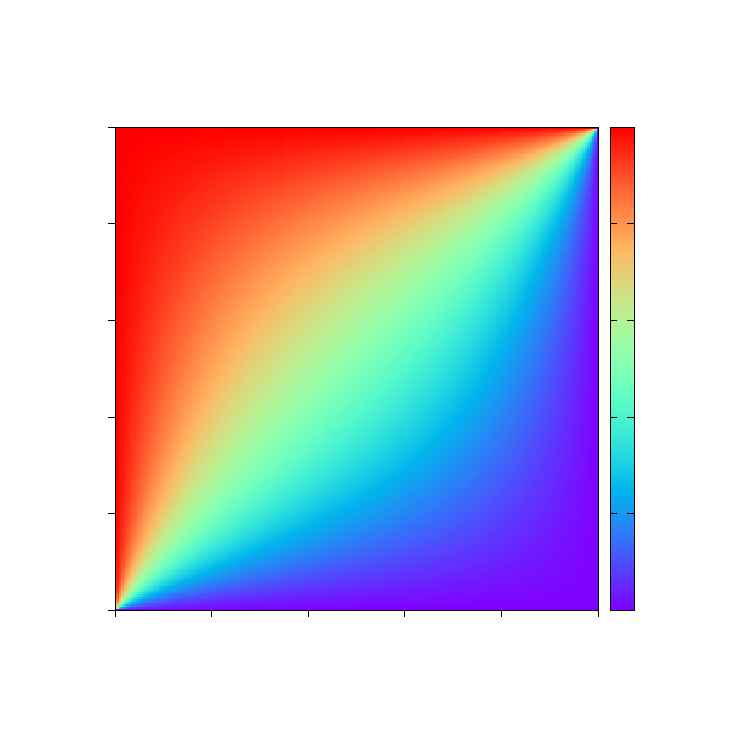
\includegraphics[width={340.10bp},height={340.10bp}]{standalone/case_diagonal_flow/diagonal_N200_Pe1.0e-01-inc}}%
    \gplfronttext
  \end{picture}%
\endgroup
\end{document}

		\vspace{-0.50cm}
		\captionsetup{width=0.8\textwidth}
		\caption{Numerical solution to the diagonal case for $\peclet = 10^{-1}$.}
		\label{fig:diagonal_N200_Pe1.0e-01}
	\end{subfigure}%
	\begin{subfigure}{.5\textwidth}
		\centering
		\vspace{-0.75cm}
		%		\fbox{% GNUPLOT: LaTeX picture with Postscript
\documentclass{minimal}
% Set font size
\makeatletter
\def\@ptsize{1}
\InputIfFileExists{size11.clo}{}{%
   \GenericError{(gnuplot) \space\space\space\@spaces}{%
      Gnuplot Error: File `size11.clo' not found! Could not set font size%
   }{See the gnuplot documentation for explanation.%
   }{For using a font size a file `size<fontsize>.clo' has to exist.
        Falling back ^^Jto default fontsize 10pt.}%
  \def\@ptsize{0}
  \input{size10.clo}%
}%
\makeatother
% Load packages
\usepackage{calc}
\usepackage{graphicx}
\usepackage{color}
\usepackage[cp1252]{inputenc}
\makeatletter
% Select an appropriate default driver (from TeXLive graphics.cfg)
\begingroup
  \chardef\x=0 %
  % check pdfTeX
  \@ifundefined{pdfoutput}{}{%
    \ifcase\pdfoutput
    \else
      \chardef\x=1 %
    \fi
  }%
  % check VTeX
  \@ifundefined{OpMode}{}{%
    \chardef\x=2 %
  }%
\expandafter\endgroup
\ifcase\x
  % default case
  \PassOptionsToPackage{dvips}{geometry}
\or
  % pdfTeX is running in pdf mode
  \PassOptionsToPackage{pdftex}{geometry}
\else
  % VTeX is running
  \PassOptionsToPackage{vtex}{geometry}
\fi
\makeatother
% Set papersize
\usepackage[papersize={340.10bp,340.10bp},text={340.10bp,340.10bp}]{geometry}
% No page numbers and no paragraph indentation
\pagestyle{empty}
\setlength{\parindent}{0bp}%
% Load configuration file
\InputIfFileExists{gnuplot.cfg}{%
  \typeout{Using configuration file gnuplot.cfg}%
}{%
 \typeout{No configuration file gnuplot.cfg found.}%
}%
%
\begin{document}
\begingroup
  % Encoding inside the plot.  In the header of your document, this encoding
  % should to defined, e.g., by using
  % \usepackage[cp1252,<other encodings>]{inputenc}
  \inputencoding{cp1252}%
  \makeatletter
  \providecommand\color[2][]{%
    \GenericError{(gnuplot) \space\space\space\@spaces}{%
      Package color not loaded in conjunction with
      terminal option `colourtext'%
    }{See the gnuplot documentation for explanation.%
    }{Either use 'blacktext' in gnuplot or load the package
      color.sty in LaTeX.}%
    \renewcommand\color[2][]{}%
  }%
  \providecommand\includegraphics[2][]{%
    \GenericError{(gnuplot) \space\space\space\@spaces}{%
      Package graphicx or graphics not loaded%
    }{See the gnuplot documentation for explanation.%
    }{The gnuplot epslatex terminal needs graphicx.sty or graphics.sty.}%
    \renewcommand\includegraphics[2][]{}%
  }%
  \providecommand\rotatebox[2]{#2}%
  \@ifundefined{ifGPcolor}{%
    \newif\ifGPcolor
    \GPcolortrue
  }{}%
  \@ifundefined{ifGPblacktext}{%
    \newif\ifGPblacktext
    \GPblacktextfalse
  }{}%
  % define a \g@addto@macro without @ in the name:
  \let\gplgaddtomacro\g@addto@macro
  % define empty templates for all commands taking text:
  \gdef\gplbacktext{}%
  \gdef\gplfronttext{}%
  \makeatother
  \ifGPblacktext
    % no textcolor at all
    \def\colorrgb#1{}%
    \def\colorgray#1{}%
  \else
    % gray or color?
    \ifGPcolor
      \def\colorrgb#1{\color[rgb]{#1}}%
      \def\colorgray#1{\color[gray]{#1}}%
      \expandafter\def\csname LTw\endcsname{\color{white}}%
      \expandafter\def\csname LTb\endcsname{\color{black}}%
      \expandafter\def\csname LTa\endcsname{\color{black}}%
      \expandafter\def\csname LT0\endcsname{\color[rgb]{1,0,0}}%
      \expandafter\def\csname LT1\endcsname{\color[rgb]{0,1,0}}%
      \expandafter\def\csname LT2\endcsname{\color[rgb]{0,0,1}}%
      \expandafter\def\csname LT3\endcsname{\color[rgb]{1,0,1}}%
      \expandafter\def\csname LT4\endcsname{\color[rgb]{0,1,1}}%
      \expandafter\def\csname LT5\endcsname{\color[rgb]{1,1,0}}%
      \expandafter\def\csname LT6\endcsname{\color[rgb]{0,0,0}}%
      \expandafter\def\csname LT7\endcsname{\color[rgb]{1,0.3,0}}%
      \expandafter\def\csname LT8\endcsname{\color[rgb]{0.5,0.5,0.5}}%
    \else
      % gray
      \def\colorrgb#1{\color{black}}%
      \def\colorgray#1{\color[gray]{#1}}%
      \expandafter\def\csname LTw\endcsname{\color{white}}%
      \expandafter\def\csname LTb\endcsname{\color{black}}%
      \expandafter\def\csname LTa\endcsname{\color{black}}%
      \expandafter\def\csname LT0\endcsname{\color{black}}%
      \expandafter\def\csname LT1\endcsname{\color{black}}%
      \expandafter\def\csname LT2\endcsname{\color{black}}%
      \expandafter\def\csname LT3\endcsname{\color{black}}%
      \expandafter\def\csname LT4\endcsname{\color{black}}%
      \expandafter\def\csname LT5\endcsname{\color{black}}%
      \expandafter\def\csname LT6\endcsname{\color{black}}%
      \expandafter\def\csname LT7\endcsname{\color{black}}%
      \expandafter\def\csname LT8\endcsname{\color{black}}%
    \fi
  \fi
    \setlength{\unitlength}{0.0500bp}%
    \ifx\gptboxheight\undefined%
      \newlength{\gptboxheight}%
      \newlength{\gptboxwidth}%
      \newsavebox{\gptboxtext}%
    \fi%
    \setlength{\fboxrule}{0.5pt}%
    \setlength{\fboxsep}{1pt}%
    \definecolor{tbcol}{rgb}{1,1,1}%
\begin{picture}(6802.00,6802.00)%
    \gplgaddtomacro\gplbacktext{%
      \csname LTb\endcsname%%
      \put(814,1105){\makebox(0,0)[r]{\strut{}0.0}}%
      \put(814,2032){\makebox(0,0)[r]{\strut{}0.2}}%
      \put(814,2959){\makebox(0,0)[r]{\strut{}0.4}}%
      \put(814,3886){\makebox(0,0)[r]{\strut{}0.6}}%
      \put(814,4813){\makebox(0,0)[r]{\strut{}0.8}}%
      \put(814,5740){\makebox(0,0)[r]{\strut{}1.0}}%
      \put(946,885){\makebox(0,0){\strut{}0.0}}%
      \put(1873,885){\makebox(0,0){\strut{}0.2}}%
      \put(2800,885){\makebox(0,0){\strut{}0.4}}%
      \put(3727,885){\makebox(0,0){\strut{}0.6}}%
      \put(4654,885){\makebox(0,0){\strut{}0.8}}%
      \put(5581,885){\makebox(0,0){\strut{}1.0}}%
    }%
    \gplgaddtomacro\gplfronttext{%
      \csname LTb\endcsname%%
      \put(209,3422){\rotatebox{-270}{\makebox(0,0){\strut{}$y \ (\mathrm{m})$}}}%
      \put(3263,555){\makebox(0,0){\strut{}$x \ (\mathrm{m})$}}%
      \csname LTb\endcsname%%
      \put(6060,1105){\makebox(0,0)[l]{\strut{}0.0}}%
      \put(6060,2032){\makebox(0,0)[l]{\strut{}0.2}}%
      \put(6060,2959){\makebox(0,0)[l]{\strut{}0.4}}%
      \put(6060,3886){\makebox(0,0)[l]{\strut{}0.6}}%
      \put(6060,4813){\makebox(0,0)[l]{\strut{}0.8}}%
      \put(6060,5740){\makebox(0,0)[l]{\strut{}1.0}}%
      \put(6522,3422){\rotatebox{-270}{\makebox(0,0){\strut{}$\phi$}}}%
      \put(3263,6070){\makebox(0,0){\strut{}\textbf{Diagonal case} $(\mathrm{Pe} = 10^{-2})$}}%
    }%
    \gplbacktext
    \put(0,0){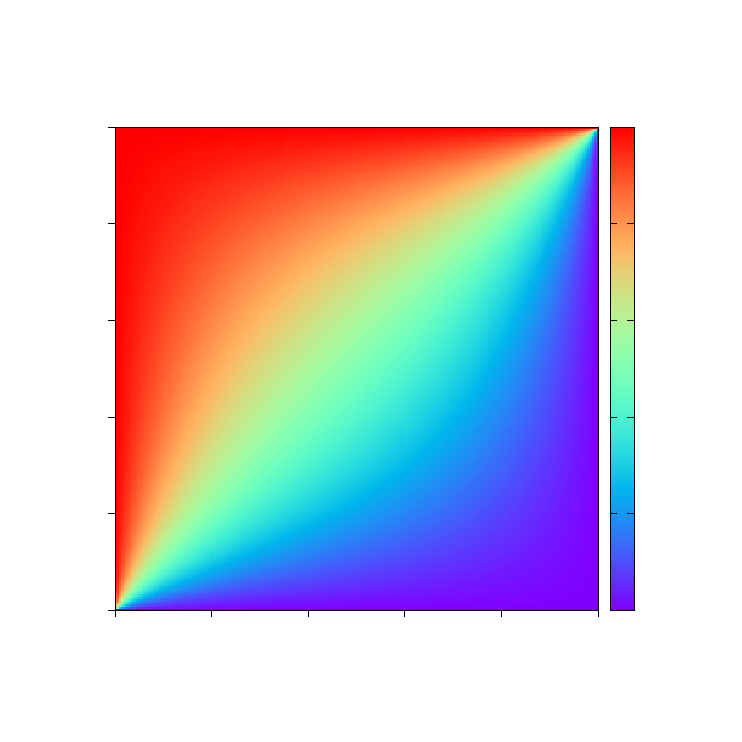
\includegraphics[width={340.10bp},height={340.10bp}]{diagonal_N200_Pe1.0e-02-inc}}%
    \gplfronttext
  \end{picture}%
\endgroup
\end{document}
}
		% GNUPLOT: LaTeX picture with Postscript
\documentclass{minimal}
% Set font size
\makeatletter
\def\@ptsize{1}
\InputIfFileExists{size11.clo}{}{%
   \GenericError{(gnuplot) \space\space\space\@spaces}{%
      Gnuplot Error: File `size11.clo' not found! Could not set font size%
   }{See the gnuplot documentation for explanation.%
   }{For using a font size a file `size<fontsize>.clo' has to exist.
        Falling back ^^Jto default fontsize 10pt.}%
  \def\@ptsize{0}
  \input{size10.clo}%
}%
\makeatother
% Load packages
\usepackage{calc}
\usepackage{graphicx}
\usepackage{color}
\usepackage[cp1252]{inputenc}
\makeatletter
% Select an appropriate default driver (from TeXLive graphics.cfg)
\begingroup
  \chardef\x=0 %
  % check pdfTeX
  \@ifundefined{pdfoutput}{}{%
    \ifcase\pdfoutput
    \else
      \chardef\x=1 %
    \fi
  }%
  % check VTeX
  \@ifundefined{OpMode}{}{%
    \chardef\x=2 %
  }%
\expandafter\endgroup
\ifcase\x
  % default case
  \PassOptionsToPackage{dvips}{geometry}
\or
  % pdfTeX is running in pdf mode
  \PassOptionsToPackage{pdftex}{geometry}
\else
  % VTeX is running
  \PassOptionsToPackage{vtex}{geometry}
\fi
\makeatother
% Set papersize
\usepackage[papersize={340.10bp,340.10bp},text={340.10bp,340.10bp}]{geometry}
% No page numbers and no paragraph indentation
\pagestyle{empty}
\setlength{\parindent}{0bp}%
% Load configuration file
\InputIfFileExists{gnuplot.cfg}{%
  \typeout{Using configuration file gnuplot.cfg}%
}{%
 \typeout{No configuration file gnuplot.cfg found.}%
}%
%
\begin{document}
\begingroup
  % Encoding inside the plot.  In the header of your document, this encoding
  % should to defined, e.g., by using
  % \usepackage[cp1252,<other encodings>]{inputenc}
  \inputencoding{cp1252}%
  \makeatletter
  \providecommand\color[2][]{%
    \GenericError{(gnuplot) \space\space\space\@spaces}{%
      Package color not loaded in conjunction with
      terminal option `colourtext'%
    }{See the gnuplot documentation for explanation.%
    }{Either use 'blacktext' in gnuplot or load the package
      color.sty in LaTeX.}%
    \renewcommand\color[2][]{}%
  }%
  \providecommand\includegraphics[2][]{%
    \GenericError{(gnuplot) \space\space\space\@spaces}{%
      Package graphicx or graphics not loaded%
    }{See the gnuplot documentation for explanation.%
    }{The gnuplot epslatex terminal needs graphicx.sty or graphics.sty.}%
    \renewcommand\includegraphics[2][]{}%
  }%
  \providecommand\rotatebox[2]{#2}%
  \@ifundefined{ifGPcolor}{%
    \newif\ifGPcolor
    \GPcolortrue
  }{}%
  \@ifundefined{ifGPblacktext}{%
    \newif\ifGPblacktext
    \GPblacktextfalse
  }{}%
  % define a \g@addto@macro without @ in the name:
  \let\gplgaddtomacro\g@addto@macro
  % define empty templates for all commands taking text:
  \gdef\gplbacktext{}%
  \gdef\gplfronttext{}%
  \makeatother
  \ifGPblacktext
    % no textcolor at all
    \def\colorrgb#1{}%
    \def\colorgray#1{}%
  \else
    % gray or color?
    \ifGPcolor
      \def\colorrgb#1{\color[rgb]{#1}}%
      \def\colorgray#1{\color[gray]{#1}}%
      \expandafter\def\csname LTw\endcsname{\color{white}}%
      \expandafter\def\csname LTb\endcsname{\color{black}}%
      \expandafter\def\csname LTa\endcsname{\color{black}}%
      \expandafter\def\csname LT0\endcsname{\color[rgb]{1,0,0}}%
      \expandafter\def\csname LT1\endcsname{\color[rgb]{0,1,0}}%
      \expandafter\def\csname LT2\endcsname{\color[rgb]{0,0,1}}%
      \expandafter\def\csname LT3\endcsname{\color[rgb]{1,0,1}}%
      \expandafter\def\csname LT4\endcsname{\color[rgb]{0,1,1}}%
      \expandafter\def\csname LT5\endcsname{\color[rgb]{1,1,0}}%
      \expandafter\def\csname LT6\endcsname{\color[rgb]{0,0,0}}%
      \expandafter\def\csname LT7\endcsname{\color[rgb]{1,0.3,0}}%
      \expandafter\def\csname LT8\endcsname{\color[rgb]{0.5,0.5,0.5}}%
    \else
      % gray
      \def\colorrgb#1{\color{black}}%
      \def\colorgray#1{\color[gray]{#1}}%
      \expandafter\def\csname LTw\endcsname{\color{white}}%
      \expandafter\def\csname LTb\endcsname{\color{black}}%
      \expandafter\def\csname LTa\endcsname{\color{black}}%
      \expandafter\def\csname LT0\endcsname{\color{black}}%
      \expandafter\def\csname LT1\endcsname{\color{black}}%
      \expandafter\def\csname LT2\endcsname{\color{black}}%
      \expandafter\def\csname LT3\endcsname{\color{black}}%
      \expandafter\def\csname LT4\endcsname{\color{black}}%
      \expandafter\def\csname LT5\endcsname{\color{black}}%
      \expandafter\def\csname LT6\endcsname{\color{black}}%
      \expandafter\def\csname LT7\endcsname{\color{black}}%
      \expandafter\def\csname LT8\endcsname{\color{black}}%
    \fi
  \fi
    \setlength{\unitlength}{0.0500bp}%
    \ifx\gptboxheight\undefined%
      \newlength{\gptboxheight}%
      \newlength{\gptboxwidth}%
      \newsavebox{\gptboxtext}%
    \fi%
    \setlength{\fboxrule}{0.5pt}%
    \setlength{\fboxsep}{1pt}%
    \definecolor{tbcol}{rgb}{1,1,1}%
\begin{picture}(6802.00,6802.00)%
    \gplgaddtomacro\gplbacktext{%
      \csname LTb\endcsname%%
      \put(814,1105){\makebox(0,0)[r]{\strut{}0.0}}%
      \put(814,2032){\makebox(0,0)[r]{\strut{}0.2}}%
      \put(814,2959){\makebox(0,0)[r]{\strut{}0.4}}%
      \put(814,3886){\makebox(0,0)[r]{\strut{}0.6}}%
      \put(814,4813){\makebox(0,0)[r]{\strut{}0.8}}%
      \put(814,5740){\makebox(0,0)[r]{\strut{}1.0}}%
      \put(946,885){\makebox(0,0){\strut{}0.0}}%
      \put(1873,885){\makebox(0,0){\strut{}0.2}}%
      \put(2800,885){\makebox(0,0){\strut{}0.4}}%
      \put(3727,885){\makebox(0,0){\strut{}0.6}}%
      \put(4654,885){\makebox(0,0){\strut{}0.8}}%
      \put(5581,885){\makebox(0,0){\strut{}1.0}}%
    }%
    \gplgaddtomacro\gplfronttext{%
      \csname LTb\endcsname%%
      \put(209,3422){\rotatebox{-270}{\makebox(0,0){\strut{}$y \ (\mathrm{m})$}}}%
      \put(3263,555){\makebox(0,0){\strut{}$x \ (\mathrm{m})$}}%
      \csname LTb\endcsname%%
      \put(6060,1105){\makebox(0,0)[l]{\strut{}0.0}}%
      \put(6060,2032){\makebox(0,0)[l]{\strut{}0.2}}%
      \put(6060,2959){\makebox(0,0)[l]{\strut{}0.4}}%
      \put(6060,3886){\makebox(0,0)[l]{\strut{}0.6}}%
      \put(6060,4813){\makebox(0,0)[l]{\strut{}0.8}}%
      \put(6060,5740){\makebox(0,0)[l]{\strut{}1.0}}%
      \put(6522,3422){\rotatebox{-270}{\makebox(0,0){\strut{}$\phi$}}}%
      \put(3263,6070){\makebox(0,0){\strut{}\textbf{Diagonal case} $(\mathrm{Pe} = 10^{-2})$}}%
    }%
    \gplbacktext
    \put(0,0){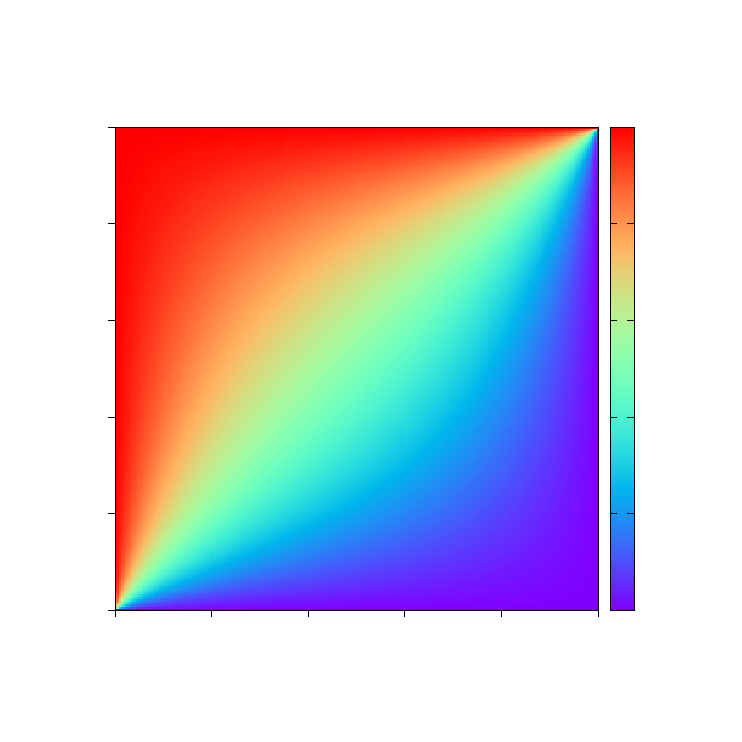
\includegraphics[width={340.10bp},height={340.10bp}]{diagonal_N200_Pe1.0e-02-inc}}%
    \gplfronttext
  \end{picture}%
\endgroup
\end{document}

		\vspace{-0.50cm}
		\captionsetup{width=0.8\textwidth}
		\caption{Numerical solution to the diagonal case for $\peclet = 10^{-2}$.}
		\label{fig:diagonal_N200_Pe1.0e-02}
	\end{subfigure}
	\begin{subfigure}{.5\textwidth}
		\centering
		\vspace{-0.25cm}
		%		\fbox{% GNUPLOT: LaTeX picture with Postscript
\begingroup
  % Encoding inside the plot.  In the header of your document, this encoding
  % should to defined, e.g., by using
  % \usepackage[cp1252,<other encodings>]{inputenc}
  \inputencoding{cp1252}%
  \makeatletter
  \providecommand\color[2][]{%
    \GenericError{(gnuplot) \space\space\space\@spaces}{%
      Package color not loaded in conjunction with
      terminal option `colourtext'%
    }{See the gnuplot documentation for explanation.%
    }{Either use 'blacktext' in gnuplot or load the package
      color.sty in LaTeX.}%
    \renewcommand\color[2][]{}%
  }%
  \providecommand\includegraphics[2][]{%
    \GenericError{(gnuplot) \space\space\space\@spaces}{%
      Package graphicx or graphics not loaded%
    }{See the gnuplot documentation for explanation.%
    }{The gnuplot epslatex terminal needs graphicx.sty or graphics.sty.}%
    \renewcommand\includegraphics[2][]{}%
  }%
  \providecommand\rotatebox[2]{#2}%
  \@ifundefined{ifGPcolor}{%
    \newif\ifGPcolor
    \GPcolortrue
  }{}%
  \@ifundefined{ifGPblacktext}{%
    \newif\ifGPblacktext
    \GPblacktextfalse
  }{}%
  % define a \g@addto@macro without @ in the name:
  \let\gplgaddtomacro\g@addto@macro
  % define empty templates for all commands taking text:
  \gdef\gplbacktext{}%
  \gdef\gplfronttext{}%
  \makeatother
  \ifGPblacktext
    % no textcolor at all
    \def\colorrgb#1{}%
    \def\colorgray#1{}%
  \else
    % gray or color?
    \ifGPcolor
      \def\colorrgb#1{\color[rgb]{#1}}%
      \def\colorgray#1{\color[gray]{#1}}%
      \expandafter\def\csname LTw\endcsname{\color{white}}%
      \expandafter\def\csname LTb\endcsname{\color{black}}%
      \expandafter\def\csname LTa\endcsname{\color{black}}%
      \expandafter\def\csname LT0\endcsname{\color[rgb]{1,0,0}}%
      \expandafter\def\csname LT1\endcsname{\color[rgb]{0,1,0}}%
      \expandafter\def\csname LT2\endcsname{\color[rgb]{0,0,1}}%
      \expandafter\def\csname LT3\endcsname{\color[rgb]{1,0,1}}%
      \expandafter\def\csname LT4\endcsname{\color[rgb]{0,1,1}}%
      \expandafter\def\csname LT5\endcsname{\color[rgb]{1,1,0}}%
      \expandafter\def\csname LT6\endcsname{\color[rgb]{0,0,0}}%
      \expandafter\def\csname LT7\endcsname{\color[rgb]{1,0.3,0}}%
      \expandafter\def\csname LT8\endcsname{\color[rgb]{0.5,0.5,0.5}}%
    \else
      % gray
      \def\colorrgb#1{\color{black}}%
      \def\colorgray#1{\color[gray]{#1}}%
      \expandafter\def\csname LTw\endcsname{\color{white}}%
      \expandafter\def\csname LTb\endcsname{\color{black}}%
      \expandafter\def\csname LTa\endcsname{\color{black}}%
      \expandafter\def\csname LT0\endcsname{\color{black}}%
      \expandafter\def\csname LT1\endcsname{\color{black}}%
      \expandafter\def\csname LT2\endcsname{\color{black}}%
      \expandafter\def\csname LT3\endcsname{\color{black}}%
      \expandafter\def\csname LT4\endcsname{\color{black}}%
      \expandafter\def\csname LT5\endcsname{\color{black}}%
      \expandafter\def\csname LT6\endcsname{\color{black}}%
      \expandafter\def\csname LT7\endcsname{\color{black}}%
      \expandafter\def\csname LT8\endcsname{\color{black}}%
    \fi
  \fi
    \setlength{\unitlength}{0.0500bp}%
    \ifx\gptboxheight\undefined%
      \newlength{\gptboxheight}%
      \newlength{\gptboxwidth}%
      \newsavebox{\gptboxtext}%
    \fi%
    \setlength{\fboxrule}{0.5pt}%
    \setlength{\fboxsep}{1pt}%
    \definecolor{tbcol}{rgb}{1,1,1}%
\begin{picture}(4534.00,4534.00)%
    \gplgaddtomacro\gplbacktext{%
      \csname LTb\endcsname%%
      \put(814,991){\makebox(0,0)[r]{\strut{}0.0}}%
      \put(814,1510){\makebox(0,0)[r]{\strut{}0.2}}%
      \put(814,2029){\makebox(0,0)[r]{\strut{}0.4}}%
      \put(814,2548){\makebox(0,0)[r]{\strut{}0.6}}%
      \put(814,3067){\makebox(0,0)[r]{\strut{}0.8}}%
      \put(814,3586){\makebox(0,0)[r]{\strut{}1.0}}%
      \put(946,771){\makebox(0,0){\strut{}0.0}}%
      \put(1465,771){\makebox(0,0){\strut{}0.2}}%
      \put(1984,771){\makebox(0,0){\strut{}0.4}}%
      \put(2502,771){\makebox(0,0){\strut{}0.6}}%
      \put(3021,771){\makebox(0,0){\strut{}0.8}}%
      \put(3540,771){\makebox(0,0){\strut{}1.0}}%
    }%
    \gplgaddtomacro\gplfronttext{%
      \csname LTb\endcsname%%
      \put(209,2288){\rotatebox{-270}{\makebox(0,0){\strut{}$y \ (\mathrm{m})$}}}%
      \put(2243,441){\makebox(0,0){\strut{}$x \ (\mathrm{m})$}}%
      \csname LTb\endcsname%%
      \put(3866,991){\makebox(0,0)[l]{\strut{}0.0}}%
      \put(3866,1510){\makebox(0,0)[l]{\strut{}0.2}}%
      \put(3866,2029){\makebox(0,0)[l]{\strut{}0.4}}%
      \put(3866,2548){\makebox(0,0)[l]{\strut{}0.6}}%
      \put(3866,3067){\makebox(0,0)[l]{\strut{}0.8}}%
      \put(3866,3586){\makebox(0,0)[l]{\strut{}1.0}}%
      \put(4328,2288){\rotatebox{-270}{\makebox(0,0){\strut{}$\phi$}}}%
      \put(2243,3916){\makebox(0,0){\strut{}\textbf{Diagonal flow} $(\mathrm{Pe} = 10^{-4})$}}%
    }%
    \gplbacktext
    \put(0,0){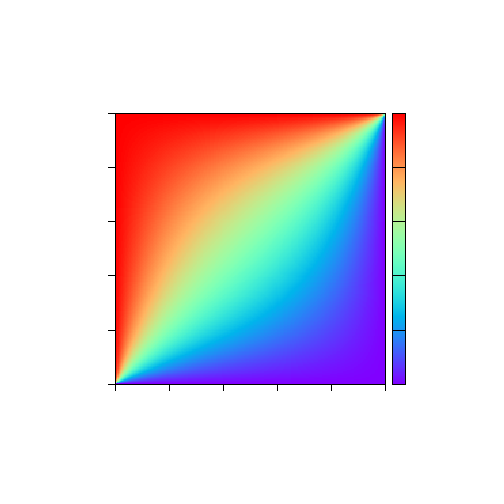
\includegraphics[width={226.70bp},height={226.70bp}]{figures/case_diagonal_flow/diagonal_N200_Pe1.0e-04}}%
    \gplfronttext
  \end{picture}%
\endgroup
}
		% GNUPLOT: LaTeX picture with Postscript
\begingroup
  % Encoding inside the plot.  In the header of your document, this encoding
  % should to defined, e.g., by using
  % \usepackage[cp1252,<other encodings>]{inputenc}
  \inputencoding{cp1252}%
  \makeatletter
  \providecommand\color[2][]{%
    \GenericError{(gnuplot) \space\space\space\@spaces}{%
      Package color not loaded in conjunction with
      terminal option `colourtext'%
    }{See the gnuplot documentation for explanation.%
    }{Either use 'blacktext' in gnuplot or load the package
      color.sty in LaTeX.}%
    \renewcommand\color[2][]{}%
  }%
  \providecommand\includegraphics[2][]{%
    \GenericError{(gnuplot) \space\space\space\@spaces}{%
      Package graphicx or graphics not loaded%
    }{See the gnuplot documentation for explanation.%
    }{The gnuplot epslatex terminal needs graphicx.sty or graphics.sty.}%
    \renewcommand\includegraphics[2][]{}%
  }%
  \providecommand\rotatebox[2]{#2}%
  \@ifundefined{ifGPcolor}{%
    \newif\ifGPcolor
    \GPcolortrue
  }{}%
  \@ifundefined{ifGPblacktext}{%
    \newif\ifGPblacktext
    \GPblacktextfalse
  }{}%
  % define a \g@addto@macro without @ in the name:
  \let\gplgaddtomacro\g@addto@macro
  % define empty templates for all commands taking text:
  \gdef\gplbacktext{}%
  \gdef\gplfronttext{}%
  \makeatother
  \ifGPblacktext
    % no textcolor at all
    \def\colorrgb#1{}%
    \def\colorgray#1{}%
  \else
    % gray or color?
    \ifGPcolor
      \def\colorrgb#1{\color[rgb]{#1}}%
      \def\colorgray#1{\color[gray]{#1}}%
      \expandafter\def\csname LTw\endcsname{\color{white}}%
      \expandafter\def\csname LTb\endcsname{\color{black}}%
      \expandafter\def\csname LTa\endcsname{\color{black}}%
      \expandafter\def\csname LT0\endcsname{\color[rgb]{1,0,0}}%
      \expandafter\def\csname LT1\endcsname{\color[rgb]{0,1,0}}%
      \expandafter\def\csname LT2\endcsname{\color[rgb]{0,0,1}}%
      \expandafter\def\csname LT3\endcsname{\color[rgb]{1,0,1}}%
      \expandafter\def\csname LT4\endcsname{\color[rgb]{0,1,1}}%
      \expandafter\def\csname LT5\endcsname{\color[rgb]{1,1,0}}%
      \expandafter\def\csname LT6\endcsname{\color[rgb]{0,0,0}}%
      \expandafter\def\csname LT7\endcsname{\color[rgb]{1,0.3,0}}%
      \expandafter\def\csname LT8\endcsname{\color[rgb]{0.5,0.5,0.5}}%
    \else
      % gray
      \def\colorrgb#1{\color{black}}%
      \def\colorgray#1{\color[gray]{#1}}%
      \expandafter\def\csname LTw\endcsname{\color{white}}%
      \expandafter\def\csname LTb\endcsname{\color{black}}%
      \expandafter\def\csname LTa\endcsname{\color{black}}%
      \expandafter\def\csname LT0\endcsname{\color{black}}%
      \expandafter\def\csname LT1\endcsname{\color{black}}%
      \expandafter\def\csname LT2\endcsname{\color{black}}%
      \expandafter\def\csname LT3\endcsname{\color{black}}%
      \expandafter\def\csname LT4\endcsname{\color{black}}%
      \expandafter\def\csname LT5\endcsname{\color{black}}%
      \expandafter\def\csname LT6\endcsname{\color{black}}%
      \expandafter\def\csname LT7\endcsname{\color{black}}%
      \expandafter\def\csname LT8\endcsname{\color{black}}%
    \fi
  \fi
    \setlength{\unitlength}{0.0500bp}%
    \ifx\gptboxheight\undefined%
      \newlength{\gptboxheight}%
      \newlength{\gptboxwidth}%
      \newsavebox{\gptboxtext}%
    \fi%
    \setlength{\fboxrule}{0.5pt}%
    \setlength{\fboxsep}{1pt}%
    \definecolor{tbcol}{rgb}{1,1,1}%
\begin{picture}(4534.00,4534.00)%
    \gplgaddtomacro\gplbacktext{%
      \csname LTb\endcsname%%
      \put(814,991){\makebox(0,0)[r]{\strut{}0.0}}%
      \put(814,1510){\makebox(0,0)[r]{\strut{}0.2}}%
      \put(814,2029){\makebox(0,0)[r]{\strut{}0.4}}%
      \put(814,2548){\makebox(0,0)[r]{\strut{}0.6}}%
      \put(814,3067){\makebox(0,0)[r]{\strut{}0.8}}%
      \put(814,3586){\makebox(0,0)[r]{\strut{}1.0}}%
      \put(946,771){\makebox(0,0){\strut{}0.0}}%
      \put(1465,771){\makebox(0,0){\strut{}0.2}}%
      \put(1984,771){\makebox(0,0){\strut{}0.4}}%
      \put(2502,771){\makebox(0,0){\strut{}0.6}}%
      \put(3021,771){\makebox(0,0){\strut{}0.8}}%
      \put(3540,771){\makebox(0,0){\strut{}1.0}}%
    }%
    \gplgaddtomacro\gplfronttext{%
      \csname LTb\endcsname%%
      \put(209,2288){\rotatebox{-270}{\makebox(0,0){\strut{}$y \ (\mathrm{m})$}}}%
      \put(2243,441){\makebox(0,0){\strut{}$x \ (\mathrm{m})$}}%
      \csname LTb\endcsname%%
      \put(3866,991){\makebox(0,0)[l]{\strut{}0.0}}%
      \put(3866,1510){\makebox(0,0)[l]{\strut{}0.2}}%
      \put(3866,2029){\makebox(0,0)[l]{\strut{}0.4}}%
      \put(3866,2548){\makebox(0,0)[l]{\strut{}0.6}}%
      \put(3866,3067){\makebox(0,0)[l]{\strut{}0.8}}%
      \put(3866,3586){\makebox(0,0)[l]{\strut{}1.0}}%
      \put(4328,2288){\rotatebox{-270}{\makebox(0,0){\strut{}$\phi$}}}%
      \put(2243,3916){\makebox(0,0){\strut{}\textbf{Diagonal flow} $(\mathrm{Pe} = 10^{-4})$}}%
    }%
    \gplbacktext
    \put(0,0){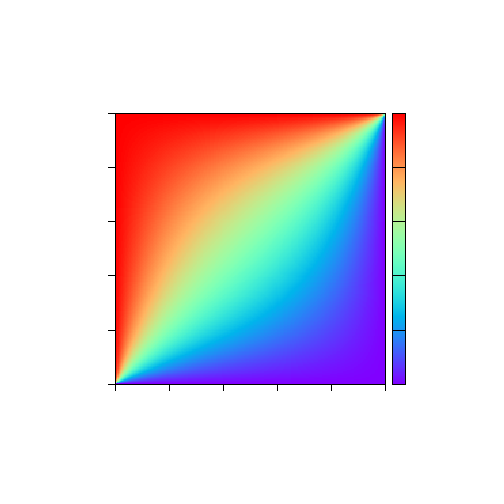
\includegraphics[width={226.70bp},height={226.70bp}]{figures/case_diagonal_flow/diagonal_N200_Pe1.0e-04}}%
    \gplfronttext
  \end{picture}%
\endgroup

		\vspace{-0.50cm}
		\captionsetup{width=0.8\textwidth}
		\caption{Numerical solution to the diagonal case for $\peclet = 10^{-4}$.}
		\label{fig:diagonal_N200_Pe1.0e-04}
	\end{subfigure}%
	\begin{subfigure}{.5\textwidth}
		\centering
		\vspace{-0.25cm}
		%		\fbox{% GNUPLOT: LaTeX picture with Postscript
\documentclass{minimal}
% Set font size
\makeatletter
\def\@ptsize{1}
\InputIfFileExists{size11.clo}{}{%
   \GenericError{(gnuplot) \space\space\space\@spaces}{%
      Gnuplot Error: File `size11.clo' not found! Could not set font size%
   }{See the gnuplot documentation for explanation.%
   }{For using a font size a file `size<fontsize>.clo' has to exist.
        Falling back ^^Jto default fontsize 10pt.}%
  \def\@ptsize{0}
  \input{size10.clo}%
}%
\makeatother
% Load packages
\usepackage{calc}
\usepackage{graphicx}
\usepackage{color}
\usepackage[cp1252]{inputenc}
\makeatletter
% Select an appropriate default driver (from TeXLive graphics.cfg)
\begingroup
  \chardef\x=0 %
  % check pdfTeX
  \@ifundefined{pdfoutput}{}{%
    \ifcase\pdfoutput
    \else
      \chardef\x=1 %
    \fi
  }%
  % check VTeX
  \@ifundefined{OpMode}{}{%
    \chardef\x=2 %
  }%
\expandafter\endgroup
\ifcase\x
  % default case
  \PassOptionsToPackage{dvips}{geometry}
\or
  % pdfTeX is running in pdf mode
  \PassOptionsToPackage{pdftex}{geometry}
\else
  % VTeX is running
  \PassOptionsToPackage{vtex}{geometry}
\fi
\makeatother
% Set papersize
\usepackage[papersize={340.10bp,340.10bp},text={340.10bp,340.10bp}]{geometry}
% No page numbers and no paragraph indentation
\pagestyle{empty}
\setlength{\parindent}{0bp}%
% Load configuration file
\InputIfFileExists{gnuplot.cfg}{%
  \typeout{Using configuration file gnuplot.cfg}%
}{%
 \typeout{No configuration file gnuplot.cfg found.}%
}%
%
\begin{document}
\begingroup
  % Encoding inside the plot.  In the header of your document, this encoding
  % should to defined, e.g., by using
  % \usepackage[cp1252,<other encodings>]{inputenc}
  \inputencoding{cp1252}%
  \makeatletter
  \providecommand\color[2][]{%
    \GenericError{(gnuplot) \space\space\space\@spaces}{%
      Package color not loaded in conjunction with
      terminal option `colourtext'%
    }{See the gnuplot documentation for explanation.%
    }{Either use 'blacktext' in gnuplot or load the package
      color.sty in LaTeX.}%
    \renewcommand\color[2][]{}%
  }%
  \providecommand\includegraphics[2][]{%
    \GenericError{(gnuplot) \space\space\space\@spaces}{%
      Package graphicx or graphics not loaded%
    }{See the gnuplot documentation for explanation.%
    }{The gnuplot epslatex terminal needs graphicx.sty or graphics.sty.}%
    \renewcommand\includegraphics[2][]{}%
  }%
  \providecommand\rotatebox[2]{#2}%
  \@ifundefined{ifGPcolor}{%
    \newif\ifGPcolor
    \GPcolortrue
  }{}%
  \@ifundefined{ifGPblacktext}{%
    \newif\ifGPblacktext
    \GPblacktextfalse
  }{}%
  % define a \g@addto@macro without @ in the name:
  \let\gplgaddtomacro\g@addto@macro
  % define empty templates for all commands taking text:
  \gdef\gplbacktext{}%
  \gdef\gplfronttext{}%
  \makeatother
  \ifGPblacktext
    % no textcolor at all
    \def\colorrgb#1{}%
    \def\colorgray#1{}%
  \else
    % gray or color?
    \ifGPcolor
      \def\colorrgb#1{\color[rgb]{#1}}%
      \def\colorgray#1{\color[gray]{#1}}%
      \expandafter\def\csname LTw\endcsname{\color{white}}%
      \expandafter\def\csname LTb\endcsname{\color{black}}%
      \expandafter\def\csname LTa\endcsname{\color{black}}%
      \expandafter\def\csname LT0\endcsname{\color[rgb]{1,0,0}}%
      \expandafter\def\csname LT1\endcsname{\color[rgb]{0,1,0}}%
      \expandafter\def\csname LT2\endcsname{\color[rgb]{0,0,1}}%
      \expandafter\def\csname LT3\endcsname{\color[rgb]{1,0,1}}%
      \expandafter\def\csname LT4\endcsname{\color[rgb]{0,1,1}}%
      \expandafter\def\csname LT5\endcsname{\color[rgb]{1,1,0}}%
      \expandafter\def\csname LT6\endcsname{\color[rgb]{0,0,0}}%
      \expandafter\def\csname LT7\endcsname{\color[rgb]{1,0.3,0}}%
      \expandafter\def\csname LT8\endcsname{\color[rgb]{0.5,0.5,0.5}}%
    \else
      % gray
      \def\colorrgb#1{\color{black}}%
      \def\colorgray#1{\color[gray]{#1}}%
      \expandafter\def\csname LTw\endcsname{\color{white}}%
      \expandafter\def\csname LTb\endcsname{\color{black}}%
      \expandafter\def\csname LTa\endcsname{\color{black}}%
      \expandafter\def\csname LT0\endcsname{\color{black}}%
      \expandafter\def\csname LT1\endcsname{\color{black}}%
      \expandafter\def\csname LT2\endcsname{\color{black}}%
      \expandafter\def\csname LT3\endcsname{\color{black}}%
      \expandafter\def\csname LT4\endcsname{\color{black}}%
      \expandafter\def\csname LT5\endcsname{\color{black}}%
      \expandafter\def\csname LT6\endcsname{\color{black}}%
      \expandafter\def\csname LT7\endcsname{\color{black}}%
      \expandafter\def\csname LT8\endcsname{\color{black}}%
    \fi
  \fi
    \setlength{\unitlength}{0.0500bp}%
    \ifx\gptboxheight\undefined%
      \newlength{\gptboxheight}%
      \newlength{\gptboxwidth}%
      \newsavebox{\gptboxtext}%
    \fi%
    \setlength{\fboxrule}{0.5pt}%
    \setlength{\fboxsep}{1pt}%
    \definecolor{tbcol}{rgb}{1,1,1}%
\begin{picture}(6802.00,6802.00)%
    \gplgaddtomacro\gplbacktext{%
      \csname LTb\endcsname%%
      \put(814,1105){\makebox(0,0)[r]{\strut{}0.0}}%
      \put(814,2032){\makebox(0,0)[r]{\strut{}0.2}}%
      \put(814,2959){\makebox(0,0)[r]{\strut{}0.4}}%
      \put(814,3886){\makebox(0,0)[r]{\strut{}0.6}}%
      \put(814,4813){\makebox(0,0)[r]{\strut{}0.8}}%
      \put(814,5740){\makebox(0,0)[r]{\strut{}1.0}}%
      \put(946,885){\makebox(0,0){\strut{}0.0}}%
      \put(1873,885){\makebox(0,0){\strut{}0.2}}%
      \put(2800,885){\makebox(0,0){\strut{}0.4}}%
      \put(3727,885){\makebox(0,0){\strut{}0.6}}%
      \put(4654,885){\makebox(0,0){\strut{}0.8}}%
      \put(5581,885){\makebox(0,0){\strut{}1.0}}%
    }%
    \gplgaddtomacro\gplfronttext{%
      \csname LTb\endcsname%%
      \put(209,3422){\rotatebox{-270}{\makebox(0,0){\strut{}$y \ (\mathrm{m})$}}}%
      \put(3263,555){\makebox(0,0){\strut{}$x \ (\mathrm{m})$}}%
      \csname LTb\endcsname%%
      \put(6060,1105){\makebox(0,0)[l]{\strut{}0.0}}%
      \put(6060,2032){\makebox(0,0)[l]{\strut{}0.2}}%
      \put(6060,2959){\makebox(0,0)[l]{\strut{}0.4}}%
      \put(6060,3886){\makebox(0,0)[l]{\strut{}0.6}}%
      \put(6060,4813){\makebox(0,0)[l]{\strut{}0.8}}%
      \put(6060,5740){\makebox(0,0)[l]{\strut{}1.0}}%
      \put(6522,3422){\rotatebox{-270}{\makebox(0,0){\strut{}$\phi$}}}%
      \put(3263,6070){\makebox(0,0){\strut{}\textbf{Diagonal case} $(\mathrm{Pe} = 10^{-9})$}}%
    }%
    \gplbacktext
    \put(0,0){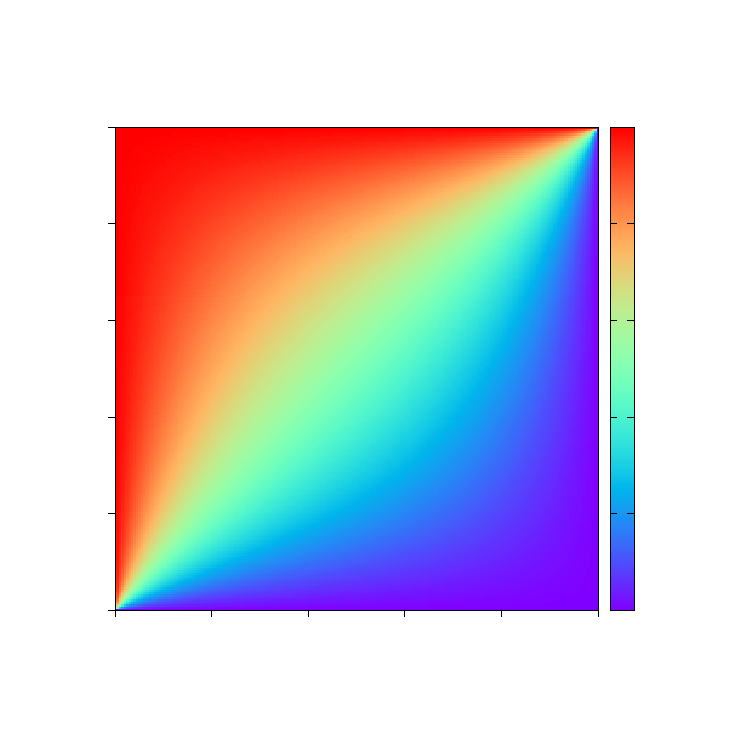
\includegraphics[width={340.10bp},height={340.10bp}]{diagonal_N200_Pe1.0e-09-inc}}%
    \gplfronttext
  \end{picture}%
\endgroup
\end{document}
}
		% GNUPLOT: LaTeX picture with Postscript
\documentclass{minimal}
% Set font size
\makeatletter
\def\@ptsize{1}
\InputIfFileExists{size11.clo}{}{%
   \GenericError{(gnuplot) \space\space\space\@spaces}{%
      Gnuplot Error: File `size11.clo' not found! Could not set font size%
   }{See the gnuplot documentation for explanation.%
   }{For using a font size a file `size<fontsize>.clo' has to exist.
        Falling back ^^Jto default fontsize 10pt.}%
  \def\@ptsize{0}
  \input{size10.clo}%
}%
\makeatother
% Load packages
\usepackage{calc}
\usepackage{graphicx}
\usepackage{color}
\usepackage[cp1252]{inputenc}
\makeatletter
% Select an appropriate default driver (from TeXLive graphics.cfg)
\begingroup
  \chardef\x=0 %
  % check pdfTeX
  \@ifundefined{pdfoutput}{}{%
    \ifcase\pdfoutput
    \else
      \chardef\x=1 %
    \fi
  }%
  % check VTeX
  \@ifundefined{OpMode}{}{%
    \chardef\x=2 %
  }%
\expandafter\endgroup
\ifcase\x
  % default case
  \PassOptionsToPackage{dvips}{geometry}
\or
  % pdfTeX is running in pdf mode
  \PassOptionsToPackage{pdftex}{geometry}
\else
  % VTeX is running
  \PassOptionsToPackage{vtex}{geometry}
\fi
\makeatother
% Set papersize
\usepackage[papersize={340.10bp,340.10bp},text={340.10bp,340.10bp}]{geometry}
% No page numbers and no paragraph indentation
\pagestyle{empty}
\setlength{\parindent}{0bp}%
% Load configuration file
\InputIfFileExists{gnuplot.cfg}{%
  \typeout{Using configuration file gnuplot.cfg}%
}{%
 \typeout{No configuration file gnuplot.cfg found.}%
}%
%
\begin{document}
\begingroup
  % Encoding inside the plot.  In the header of your document, this encoding
  % should to defined, e.g., by using
  % \usepackage[cp1252,<other encodings>]{inputenc}
  \inputencoding{cp1252}%
  \makeatletter
  \providecommand\color[2][]{%
    \GenericError{(gnuplot) \space\space\space\@spaces}{%
      Package color not loaded in conjunction with
      terminal option `colourtext'%
    }{See the gnuplot documentation for explanation.%
    }{Either use 'blacktext' in gnuplot or load the package
      color.sty in LaTeX.}%
    \renewcommand\color[2][]{}%
  }%
  \providecommand\includegraphics[2][]{%
    \GenericError{(gnuplot) \space\space\space\@spaces}{%
      Package graphicx or graphics not loaded%
    }{See the gnuplot documentation for explanation.%
    }{The gnuplot epslatex terminal needs graphicx.sty or graphics.sty.}%
    \renewcommand\includegraphics[2][]{}%
  }%
  \providecommand\rotatebox[2]{#2}%
  \@ifundefined{ifGPcolor}{%
    \newif\ifGPcolor
    \GPcolortrue
  }{}%
  \@ifundefined{ifGPblacktext}{%
    \newif\ifGPblacktext
    \GPblacktextfalse
  }{}%
  % define a \g@addto@macro without @ in the name:
  \let\gplgaddtomacro\g@addto@macro
  % define empty templates for all commands taking text:
  \gdef\gplbacktext{}%
  \gdef\gplfronttext{}%
  \makeatother
  \ifGPblacktext
    % no textcolor at all
    \def\colorrgb#1{}%
    \def\colorgray#1{}%
  \else
    % gray or color?
    \ifGPcolor
      \def\colorrgb#1{\color[rgb]{#1}}%
      \def\colorgray#1{\color[gray]{#1}}%
      \expandafter\def\csname LTw\endcsname{\color{white}}%
      \expandafter\def\csname LTb\endcsname{\color{black}}%
      \expandafter\def\csname LTa\endcsname{\color{black}}%
      \expandafter\def\csname LT0\endcsname{\color[rgb]{1,0,0}}%
      \expandafter\def\csname LT1\endcsname{\color[rgb]{0,1,0}}%
      \expandafter\def\csname LT2\endcsname{\color[rgb]{0,0,1}}%
      \expandafter\def\csname LT3\endcsname{\color[rgb]{1,0,1}}%
      \expandafter\def\csname LT4\endcsname{\color[rgb]{0,1,1}}%
      \expandafter\def\csname LT5\endcsname{\color[rgb]{1,1,0}}%
      \expandafter\def\csname LT6\endcsname{\color[rgb]{0,0,0}}%
      \expandafter\def\csname LT7\endcsname{\color[rgb]{1,0.3,0}}%
      \expandafter\def\csname LT8\endcsname{\color[rgb]{0.5,0.5,0.5}}%
    \else
      % gray
      \def\colorrgb#1{\color{black}}%
      \def\colorgray#1{\color[gray]{#1}}%
      \expandafter\def\csname LTw\endcsname{\color{white}}%
      \expandafter\def\csname LTb\endcsname{\color{black}}%
      \expandafter\def\csname LTa\endcsname{\color{black}}%
      \expandafter\def\csname LT0\endcsname{\color{black}}%
      \expandafter\def\csname LT1\endcsname{\color{black}}%
      \expandafter\def\csname LT2\endcsname{\color{black}}%
      \expandafter\def\csname LT3\endcsname{\color{black}}%
      \expandafter\def\csname LT4\endcsname{\color{black}}%
      \expandafter\def\csname LT5\endcsname{\color{black}}%
      \expandafter\def\csname LT6\endcsname{\color{black}}%
      \expandafter\def\csname LT7\endcsname{\color{black}}%
      \expandafter\def\csname LT8\endcsname{\color{black}}%
    \fi
  \fi
    \setlength{\unitlength}{0.0500bp}%
    \ifx\gptboxheight\undefined%
      \newlength{\gptboxheight}%
      \newlength{\gptboxwidth}%
      \newsavebox{\gptboxtext}%
    \fi%
    \setlength{\fboxrule}{0.5pt}%
    \setlength{\fboxsep}{1pt}%
    \definecolor{tbcol}{rgb}{1,1,1}%
\begin{picture}(6802.00,6802.00)%
    \gplgaddtomacro\gplbacktext{%
      \csname LTb\endcsname%%
      \put(814,1105){\makebox(0,0)[r]{\strut{}0.0}}%
      \put(814,2032){\makebox(0,0)[r]{\strut{}0.2}}%
      \put(814,2959){\makebox(0,0)[r]{\strut{}0.4}}%
      \put(814,3886){\makebox(0,0)[r]{\strut{}0.6}}%
      \put(814,4813){\makebox(0,0)[r]{\strut{}0.8}}%
      \put(814,5740){\makebox(0,0)[r]{\strut{}1.0}}%
      \put(946,885){\makebox(0,0){\strut{}0.0}}%
      \put(1873,885){\makebox(0,0){\strut{}0.2}}%
      \put(2800,885){\makebox(0,0){\strut{}0.4}}%
      \put(3727,885){\makebox(0,0){\strut{}0.6}}%
      \put(4654,885){\makebox(0,0){\strut{}0.8}}%
      \put(5581,885){\makebox(0,0){\strut{}1.0}}%
    }%
    \gplgaddtomacro\gplfronttext{%
      \csname LTb\endcsname%%
      \put(209,3422){\rotatebox{-270}{\makebox(0,0){\strut{}$y \ (\mathrm{m})$}}}%
      \put(3263,555){\makebox(0,0){\strut{}$x \ (\mathrm{m})$}}%
      \csname LTb\endcsname%%
      \put(6060,1105){\makebox(0,0)[l]{\strut{}0.0}}%
      \put(6060,2032){\makebox(0,0)[l]{\strut{}0.2}}%
      \put(6060,2959){\makebox(0,0)[l]{\strut{}0.4}}%
      \put(6060,3886){\makebox(0,0)[l]{\strut{}0.6}}%
      \put(6060,4813){\makebox(0,0)[l]{\strut{}0.8}}%
      \put(6060,5740){\makebox(0,0)[l]{\strut{}1.0}}%
      \put(6522,3422){\rotatebox{-270}{\makebox(0,0){\strut{}$\phi$}}}%
      \put(3263,6070){\makebox(0,0){\strut{}\textbf{Diagonal case} $(\mathrm{Pe} = 10^{-9})$}}%
    }%
    \gplbacktext
    \put(0,0){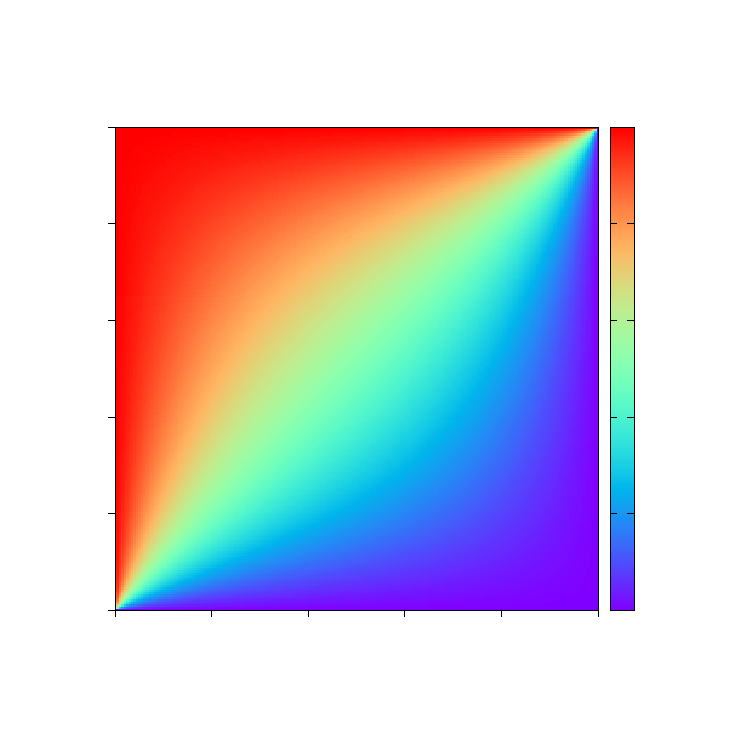
\includegraphics[width={340.10bp},height={340.10bp}]{diagonal_N200_Pe1.0e-09-inc}}%
    \gplfronttext
  \end{picture}%
\endgroup
\end{document}

		\vspace{-0.50cm}
		\captionsetup{width=0.8\textwidth}
		\caption{Numerical solution to the diagonal case for $\peclet = 10^{-9}$.}
		\label{fig:diagonal_N200_Pe1.0e-09}
	\end{subfigure}
	\caption{Numerical solution to the diagonal case for $\peclet = 10^{-1}, \ 10^{-2}, \ 10^{-4}$ and $10^{-9}$.}
	\label{fig:diagonal_N200_Pe_less_than_1}
\end{figure}